\documentclass[a4paper,12pt]{book}
%\usepackage{latexsym, amssymb}
\usepackage{amsfonts}
\usepackage{amssymb}
\usepackage{latexsym}
\usepackage{graphicx}
%\usepackage{longtable}
\usepackage{supertabular}
%\usepackage{tabularx}
%\usepackage{tabulary}
\usepackage{xspace}
\usepackage{pdfpages}
%\usepackage[rounded]{syntax}
\usepackage{hyperref} 
\usepackage{listings}
\usepackage{color} 

\usepackage[cc]{titlepic}
\usepackage{sectsty}
% \usepackage{times}
\usepackage[T1]{fontenc}
%\usepackage[urw-garamond]{mathdesign}
\usepackage{ebgaramond}
\usepackage{fncychap}
\usepackage{fancyhdr}

\usepackage{microtype}

\usepackage{rail}
\railoptions{-t -h}

\fancyhead{} % clear all header fields
\fancyheadoffset[LE,RO]{\marginparsep+\marginparwidth}
\fancyhead[RO,LE]{\thepage}
\fancyhead[LO]{\rightmark}
\fancyhead[RE]{\leftmark}
\renewcommand{\headrulewidth}{0.1pt}

\fancyfoot{}

\hypersetup{%
            colorlinks = true, %true, false
            linkcolor = black,
            citecolor = blue,
            urlcolor = blue,
}
\urlstyle{sf} %rm
\newcommand{\myurl}[1]{\textcolor{blue}{\underbar{\url{#1}}}}

%%%%%%%%%%%%%%%%%%%command imported from lac paper
\newcommand{\code}[1]	{\lstinline'#1'}
\newcommand{\OSTab}[1]	{\multicolumn{3}{|l|}{\hspace{14mm}\emph{#1}}}
\newcommand{\htab}		{\hspace*{3mm}}

%%\newcommand{\faust}		{\textsc{Faust}\xspace}
%\newcommand{\astree}	{\textsc{Astree}\xspace}
\newcommand{\grame}		{\textsc{Grame}\xspace}
\newcommand{\cierec}	{\textsc{Cierec}\xspace}
%\newcommand{\ircam}		{\textsc{Ircam}\xspace}
\newcommand{\ccrma}		{\textsc{Ccrma}\xspace}
\newcommand{\cnmat}		{\textsc{Cnmat}\xspace}
\newcommand{\create}	{\textsc{Create}\xspace}
\newcommand{\mines}		{\textsc{Mines} ParisTech\xspace}
%\newcommand{\svg}		{\textsc{Svg}\xspace}
\newcommand{\pdf}		{\textsc{Pdf}\xspace}
%%\newcommand{\latex}		{\LaTeX\xspace}
\newcommand{\ie}		{i.e.\ }
%%\newcommand{\myurl}[1]	{\textcolor{blue}{\underbar{\url{#1}}}}

%%%%%%%%%%%%%%%%%%%%%%%%%%%%%%%%%%%%%%%%%%%%%%%%%

%%% MY COLORS
\definecolor{yoheader}{rgb}{0.71,0.01,0.0}

%%%% margin par
\definecolor{margincolor}{rgb}{0.3,0.3,0.4} % grey red.
\definecolor{yobg}{rgb}{0.95,0.95,0.97}
\definecolor{yotxt}{rgb}{0.01,0.01,0.52}
\definecolor{mylstcmt}{rgb}{0.01,0.52,0.01} % a dark green.
%\definecolor{mylstdoc}{rgb}{0.60,0.60,0.60} % a medium grey.
\definecolor{mylstdoc}{rgb}{0.80,0.30,0.80} % a medium pink.
%\definecolor{mylsteqn}{rgb}{0.80,0.80,0.30} % a medium pink.
\definecolor{mylstkey}{rgb}{0.52,0.01,0.01} % a dark red.
%%\newcommand{\farg}[1]{\textrm{\textit{#1}}}

\setlength{\marginparwidth}{1.2in}
\let\oldmarginpar\marginpar
\renewcommand\marginpar[1]{\-\oldmarginpar[\raggedleft\color{margincolor}\footnotesize #1]%
{\raggedright\color{margincolor}\footnotesize #1}}

% \relax

\begin{document} 
\ChRuleWidth{1pt}
% \ChNumVar{\raggedleft\fontsize{80}{82}\sffamily\bfseries\color{yoheader}}
\ChNumVar{\raggedleft\Huge\color{yoheader}}
%\ChTitleVar{\raggedleft\fontsize{60}{62}\sffamily\it\color{yoheader}}
\ChTitleVar{\raggedleft\sffamily\fontsize{30}{32}\bf\color{yoheader}}

%\chapterfont{\sffamily\color{yoheader}}
%\sectionfont{\sffamily\color{yoheader}}
%\subsectionfont{\sffamily\color{yoheader}}
%\subsubsectionfont{\sffamily\color{yoheader}}

\chapterfont{\color{yoheader}}
\sectionfont{\color{yoheader}}
\subsectionfont{\color{yoheader}}
\subsubsectionfont{\color{yoheader}}

% parameters for listings
\lstset{
  tabsize=4,
  showspaces=false,
  showstringspaces=false,
  language=C++, 
  basicstyle=\ttfamily\color{yotxt},
  numbers=none,
  stepnumber=2,
  commentstyle=\slshape\color{mylstcmt},
  breaklines=true, 
  emph={component, declare, environment, import, library, process},
  emph={[2]ffunction, fconstant, fvariable},
  emph={[3]button, checkbox, vslider, hslider, nentry, vgroup, hgroup, tgroup, vbargraph, hbargraph, attach},
  emphstyle=\color{mylstkey},
%  morecomment=[s][\color{mylsteqn}]{<equation>}{</equation>},
  morecomment=[s][\color{mylstdoc}]{<mdoc>}{</mdoc>},
  %% frame=single,
  backgroundcolor=\color{yobg},
  captionpos=b
}

\lstloadlanguages{C++,[LaTeX]TeX}

% \titlepic{
%   \includegraphics[width=15cm]{images/bandeau-faust}
% }2.5.24.10.5
\title{\Huge\color{yoheader}FAUST Quick Reference\\\Large(version 2.5.24)}
\author{\textsc{GRAME}\\Centre National de Cr\'eation Musicale}
\date{March 2018}

\railalias{recur}{$\sim$}
\railalias{lbrace}{\{}
\railalias{rbrace}{\}}
\railalias{dollar}{\$}
\railalias{mod}{\%}
\railalias{arobase}{@}
\railalias{ampersand}{\&}
\railalias{hat}{$\land$}
\railalias{kot}{'}
\railalias{pipe}{$|$}
\railalias{fdelay}{}
\railalias{backslash}{\char"5C}
\railterm{recur,lbrace,rbrace,dollar,mod,kot,arobase,ampersand,backslash,fdelay, pipe, hat}

\newcommand{\farg}[1]{\textrm{\textit{#1}}}
\newcommand{\ldbrack}{[\![ \,}
\newcommand{\rdbrack}{\, ]\!] }
\newcommand{\rdbrackC}{\rdbrack_{\mathrm{C}}\,}
\newcommand{\dbrack}[1]{\ldbrack #1 \rdbrack}
\newcommand{\semantic}[1]{\ldbrack #1 \rdbrack}
\newcommand{\dbrackC}[1]{\ldbrack #1 \rdbrackC}

\newcommand{\faust}{\textsc{Faust}\xspace}
\newcommand{\latex}{\LaTeX\xspace}
\newcommand{\ircam}{\textsc{Ircam}\xspace}
\newcommand{\astree}{\textsc{Astree}\xspace}
\newcommand{\svg}{\textsc{Svg}\xspace}
 

\setlength{\parindent}{0pt}
\setlength{\parskip}{1ex plus 0.5ex minus 0.2ex}

\maketitle

\tableofcontents

%%%%%%%%%%%%%%%%%%%%%%%%%%%%%%%%%%%%%%%%%%%%%%%%%%%%%%%%%%%%%%%%%%%%%%%%%%%%%%%%%%%%%%
%%%%%%%%%%%%%%%%%%%%%%%%%%%%%%%%%%%%%%%%%%%%%%%%%%%%%%%%%%%%%%%%%%%%%%%%%%%%%%%%%%%%%%
%                            		CHAPTERS                                        %
%%%%%%%%%%%%%%%%%%%%%%%%%%%%%%%%%%%%%%%%%%%%%%%%%%%%%%%%%%%%%%%%%%%%%%%%%%%%%%%%%%%%%%
%%%%%%%%%%%%%%%%%%%%%%%%%%%%%%%%%%%%%%%%%%%%%%%%%%%%%%%%%%%%%%%%%%%%%%%%%%%%%%%%%%%%%%

\chapter{Introduction}
\label{chap:intro}
If you wanted to add some sound to your robot, or if you wanted to use your sound applications 
on a robot, it is now possible with \faust and the \lstinline'faust2ros' and
\lstinline'faust2rosgtk' commands. \\
\faust (\textit{Functional Audio Stream}) is a functional programming language specifically 
designed for real-time signal processing and synthesis.  \faust targets high-performance signal 
processing applications and audio plug-ins for a variety of platforms and standards.\newline
\ros (\textit{Robot Operating System}) is a flexible framework for robot software writing. It 
is a collection of tools, libraries, and conventions that aim to simplify the task of creating 
complex and robust robot behavior across a wide variety of robotic platforms.


\section{FAUST} 
\subsection{Design Principles}

Various principles have guided the design of \faust :

\begin{itemize}

\item \faust is a \textit{specification language}. It aims at providing an adequate notation to describe \textit{signal processors} from a mathematical point of view. \faust is, as much as possible, free from implementation details. 

\item \faust programs are fully compiled, not interpreted. The compiler translates \faust programs into equivalent C++ programs taking care of generating the most efficient code. The result can generally compete with, and sometimes even outperform, C++ code written by seasoned programmers. 

\item The generated code works at the sample level. It is therefore suited to implement low-level DSP functions like recursive filters. Moreover the code can be easily embedded. It is self-contained and doesn't depend of any DSP library or runtime system. It has a very deterministic behavior and a constant memory footprint. 

\item The semantic of \faust is simple and well defined. This is not just of academic interest. It allows the \faust compiler to be \emph{semantically driven}. Instead of compiling a program literally, it compiles the mathematical function it denotes. This feature is useful for example to promote components reuse while preserving optimal performance.  

\item \faust is a textual language but nevertheless block-diagram oriented. It actually combines two approaches: \textit{functional programming} and \textit{algebraic block-diagrams}. The key idea is to view block-diagram construction as function composition. For that purpose, \faust relies on a \emph{block-diagram algebra} of five composition operations (\lstinline': , ~ <: :>').

\item Thanks to the notion of \textit{architecture}, \faust programs can be easily deployed on a large variety of audio platforms and plugin formats without any change to the \faust code.

\end{itemize}

\subsection{Signal Processor Semantic}
A \faust program describes a \emph{signal processor}. 
The role of a \textit{signal processor} is to transform a group  of (possibly empty) \emph{input signals} in order to produce a group of (possibly empty) \emph{output signals}. 
Most audio equipment can be modeled as \emph{signal processors}. 
They have audio inputs, audio outputs as well as control signals interfaced with sliders, knobs, vu-meters, etc... \\

For more information about \faust, please see \textit{faust-quick-reference.pdf} and the tutorials in \faust documentation.

\section{ROS}
\subsection{What is it ?}
\marginpar {This section's content (1.2 \ros) is taken from \ros documentation. It can be found on \href{http://www.ros.org}{\ros official website} and \href{http://www.wiki.ros.org }{\ros wiki}.} Creating truly robust, general-purpose robot software is \textit {hard}. From the robot's perspective, problems that seem trivial to humans often vary wildly between instances of tasks and environments. Dealing with these variations is so hard that no single individual, laboratory, or institution can hope to do it on their own. \newline

\ros is an open-source, meta-operating system for your robot. It provides the services you would expect from an operating system, including hardware abstraction, low-level device control, implementation of commonly-used functionality, message-passing between processes, and package management. It also provides tools and libraries for obtaining, building, writing, and running code across multiple computers. \newline

As a result, \ros was built from the ground up to encourage \textit{collaborative} robotics software development. For example, one laboratory might have experts in mapping indoor environments, and could contribute a world-class system for producing maps. Another group might have experts at using maps to navigate, and yet another group might have discovered a computer vision approach that works well for recognizing small objects in clutter. \ros was designed specifically for groups like these to collaborate and build upon each other's work, as is described throughout this site.\\

\subsection{Concepts}
\subsubsection{Filesystem level}
The filesystem level concepts mainly cover \ros resources that you encounter on disk, such as:

\begin{itemize}

\item \textbf{Packages} are the main unit for organizing software in \ros. 
	A package may contain \ros runtime processes (nodes), a \ros-dependent library, datasets, configuration files, or anything else that is usefully organized together. 
	Packages are the most atomic build item and release item in \ros. Meaning that the most granular thing you can build and release is a package.

\item \textbf{Metapackages} are specialized Packages which only serve to represent a group of related other packages. 


\item \textbf{Services : }
Service descriptions, stored in my\_package/srv/MyServiceType.srv, define the request and response data structures for  \href{http://wiki.ros.org/Services}{services} in \ros.

\item \textbf{Messages : }  
Message descriptions, stored in my\_package/msg/MyMessageType.msg, define the data structures for  \href{http://wiki.ros.org/Messages}{messages} sent in \ros.


\end{itemize}


\subsubsection{Computation Graph level}
The Computation Graph is the peer-to-peer network of \ros processes that are processing data together. The basic Computation Graph concepts of \ros are nodes, Master, Parameter Server, messages, services, topics, and bags, all of which provide data to the Graph in different ways.

\begin{itemize}
\item \textbf{Master : }
The \ros Master provides name registration and lookup to the rest of the Computation Graph. Without the Master, nodes would not be able to find each other, exchange messages, or invoke services.

\item \textbf{Nodes : } 
Nodes are processes that perform computation. \ros is designed to be modular at a fine-grained scale; a robot control system usually comprises many nodes. For example, one node controls a laser range-finder, one node controls the wheel motors, one node performs localization, one node performs path planning, one Node provides a graphical view of the system, and so on. A \ros node is written with the use of a \ros client \href{http://wiki.ros.org/Client\%20Libraries}{library}, such as \href{http://wiki.ros.org/roscpp}{roscpp} or \href{http://wiki.ros.org/rospy}{rospy}.

\item \textbf{Topics : } Messages are routed via a transport system with publish / subscribe semantics. A node sends out a message by publishing it to a given \href{http://wiki.ros.org/Topics}{topic}. The topic is a name that is used to identify the content of the message. A node that is interested in a certain kind of data will subscribe to the appropriate topic. There may be multiple concurrent publishers and subscribers for a single topic, and a single node may publish and/or subscribe to multiple topics. In general, publishers and subscribers are not aware of each others' existence. The idea is to decouple the production of information from its consumption. Logically, one can think of a topic as a strongly typed message bus. Each bus has a name, and anyone can connect to the bus to send or receive messages as long as they are the right type.

\item \textbf{The Parameter Server : }The Parameter Server allows data to be stored by key in a central location. It is currently part of the Master.

\item \textbf{Messages : }Nodes communicate with each other by passing \href{http://wiki.ros.org/Messages}{messages}. A message is simply a data structure, comprising typed fields. Standard primitive types (integer, floating point, boolean, etc.) are supported, as are arrays of primitive types. Messages can include arbitrarily nested structures and arrays (much like C structures).

\end{itemize}

\begin{figure}[ht!]
\centering

 \begin{tikzpicture} [remember picture]
 \node[draw=roscolor, label={[roscolor] above left:{MASTER}}, ] (master) {
 	\begin{tikzpicture}[node distance=2.5cm]
	  \node[fill=roscolor, text=white, ellipse, text width=1.5cm, align=center](n1){Node 1};	  
	  \node[fill=roscolor, text=white, ellipse, text width=1.5cm, below=of n1, align=center](n2){Node 2};
	  \node[draw=roscolor, text=roscolor, rounded corners=3pt, text width=1.5cm, right=of n1, align=center](t1){Topic 1};
	  \node[draw=roscolor, text=roscolor, rounded corners=3pt, text width=1.5cm, right=of n2, align=center](t2){Topic 2};
	  \node[fill=roscolor, text=white, ellipse, text width=1.5cm, right=of t1, align=center](n3){Node 3};
	  \node[fill=roscolor, text=white, ellipse, text width=1.5cm, below=of n3, align=center](n4){Node 4};
	  
 
	  \draw[margincolor,->, very thick] (n1) to node [sloped, midway, above] {publication} (t1);
	  \draw[margincolor,->, very thick] (n2) to node [sloped, midway, above] {publication} (t1.south west);
 	  \draw[margincolor,->, very thick] (n3) to node [sloped, midway, above] {publication} (t2.north east);
	  \draw[yoheader,->, very thick] (t1) to node [sloped, midway, above] {subscription} (n3);
 	  \draw[yoheader,->, very thick] (t2) to node [sloped, midway, above, text width=1.9cm, align=center] {subscription} (n2);
  	  \draw[yoheader,->, very thick] (t2) to node [sloped, midway, above, text width=1.9cm, align=center] {subscription} (n4);
	\end{tikzpicture}
 };
  
 \end{tikzpicture}

\caption{\ros Concepts in a Diagram }
\label{fig:ROS Concepts}
\end{figure}

\subsubsection{Names}
Names are really important in \ros. Valid names have these characteristics :
\begin{itemize}
	\item first character is an alpha character : [a-z][A-Z]
	\item subsequent characters can be alphanumeric : [a-z][A-Z][0-9], underscores : \_ or forward slash : /
	\item there is at most one forward slash : /

\end{itemize}

For more information on \ros and tutorials, please have a look to the website :
\myurl{www.wiki.ros.org}.\\
\newpage
\section{Using FAUST with ROS}
The idea of using \faust modules with \ros could be summed up in the following diagrams.

\begin{figure}[ht!]
\centering

\begin{tikzpicture} [remember picture, node distance=0.5cm]
 \node[draw, dashed, label=above:{\faust part}] (faust) { 
 	\begin{tikzpicture}
	 \node[draw, solid, text=yoheader, fill=lightgray] (dsp) {.dsp file};
	 \node[draw=yoheader, solid, ellipse, text=black, right=of dsp, text width=1.5cm, align=center](compiler) {\faust compiler};
	 \node[draw, solid, text=yoheader, fill=lightgray, above=of compiler](archfile){architecture file};
	 \draw[->, very thick, solid] (dsp)--(compiler);
	 \draw[->, very thick, solid] (archfile)--(compiler);
	 \end{tikzpicture}
 };
 \node[draw, solid, text=yoheader, fill=lightgray, right=of compiler] (cpp) {.cpp file};
 \node[draw, dashed, right=of cpp, label=above:{\ros part}] (ROS) {
	 \begin{tikzpicture}
	 
	 \node[draw=yoheader, solid, ellipse, text=black, right=of cpp] (CMake) {catkin};
	 \node[draw, solid, text=yoheader, fill=lightgray, right=of CMake, text width=2cm, align=center] (exec) {\ros executable};
	 
	 \draw[->, very thick, solid] (CMake)--(exec);
	 \end{tikzpicture}
 };
 \draw[->,very thick] (cpp.east) -- (CMake.west);
 \draw[->,very thick] (compiler.east) -- (cpp.west);
 
\end{tikzpicture}
\caption{Compilation process }
\label{fig:Compilation principle}
\end{figure}

As shown on figure~\ref{fig:Compilation principle}, the dsp file is compiled into a C++ file thanks to the \faust compiler. Then, the C++ file can be compiled with \textit{catkin} in a \ros package to create a \ros executable, that you can run with \lstinline'rosrun'.

\begin{figure}[ht!]
\centering

 \begin{tikzpicture} [remember picture]
 
%  \node[fill=faustcolor, text=white, rounded corners=3pt, text width=1.5cm, align=center](sensor topic){Robot sensors topic};
  \node[fill=roscolor, text=white, ellipse, text width=3.5cm,  align=center](process node){\large Robot Node\\ (sends sensor data)};
  \node[draw=roscolor, text=roscolor, rounded corners=3pt, text width=3cm, align=center,  right=4cm of process node](faust topic){\large A Topic};
  \node[draw=roscolor, text=roscolor, rounded corners=3pt, text width=3cm, align=center,  below=1.5cm of process node](faust topic2){\large An other Topic};
  \node[fill=faustcolor, text=white, ellipse, text width=3.5cm, below=0.9cm of faust topic, align=center, minimum height=\heightof{process node}](faust node){\large \faust Node \\(sets audio\\ parameters with messages contents)};
% \node[fill=roscolor, text=white, ellipse, text width=1.8cm, right=of faust topic2, align=center](faust node2){\faust node : signal processing};
 
% \draw[yoheader,->, very thick] (sensor topic) to node [sloped, midway, above] {subscribing} (process node);
 \draw[margincolor,->, very thick] (process node) to node [midway, above, text width=3cm, align=center] {publishes messages} (faust topic);
 \draw[margincolor,->, thick] (process node) to node [midway, left,  text width=2.5cm, align=center] {publishes \\ other messages} (faust topic2);
 \draw[yoheader,->, very thick] (faust topic) to node [ midway, right,  text width=2.5cm] {is subscribed} (faust node);
 \draw[yoheader,->, very thick] (faust topic2) to node [ midway, above,  text width=2cm] {is subscribed} (faust node);
 
 \end{tikzpicture}

\caption{Robot using \faust}
\label{fig:Use Diagram}
\end{figure}

Once the executables coming from DSP files compiled, you can run and combine them with robotic applications (figure~\ref{fig:Use Diagram}).
\newpage
\section{Audio Server}
\faust applications use the jack audio server. Make sure it is installed on your machine.
\begin{figure}[ht!]
	\centering
	\begin{tikzpicture}[remember picture, node distance=3.5cm]
	
		\node[node distance=0, label=\color{teal}{Node 1}](node1)
		{
			\begin{tikzpicture}
				\node[draw=black,text=white, fill=indigodye, text width=4cm, align=center](processing1){\ros : processing \\ and interface};
				\node[draw=black, fill=darkpastelblue, below=of processing1, text width=4cm, align=center](audio1){jack : audio server};
			\end{tikzpicture}
		};
		\node[right=of node1, node distance=0, label=\color{teal}{Node 2}](node2){
			\begin{tikzpicture}
				\node[draw=black,text=white, fill=indigodye, text width=4cm, align=center](processing2){\ros : processing \\ and interface};
				\node[draw=black, fill=darkpastelblue, below=of processing2, text width=4cm, align=center](audio2){jack : audio server};
			\end{tikzpicture}		
		};	
		 \draw[indigodye, <->, very thick, text width=3cm, align=center] (processing1.east) to node [sloped, midway, above] {nodes parameters \\ through topics} (processing2.west);
		  \draw[darkpastelblue, <->, very thick] (audio1.east) to node [sloped, midway, below, darkcerulean] {audio datas} (audio2.west);

	\end{tikzpicture}
	
	\caption{APIs used by \faust nodes}
	\label{fig: Audio server}
\end{figure}

\section{Installation}
\subsection{FAUST}
You can get \faust on the \faust website : \href{http://faust.grame.fr/index.php/downloads}
{faust.grame.fr}. Either get it on the
 \href{https://sourceforge.net/projects/faudiostream/files/}{Source Forge Project}, or browse
  the \href{https://sourceforge.net/p/faudiostream/_list/git}{\faust's git repository}.
 You also can download the ubuntu package directly by typing : 
 \lstinline'sudo apt-get install faust' (probably an outdated version).
 \subsection{ROS}
 A \ros installation guide can be found on the
  \href{http://wiki.ros.org/indigo/Installation/Ubuntu}{\ros website}.
 \subsection{Jack}
 A Jack installation layout can be found on \href{https://github.com/jackaudio/jackaudio.github.com/wiki/InstallationLayout}{Jack's github's page}. You can download it as an Ubuntu package by typing : \lstinline'sudo apt-get install jackd2'.
\chapter{Compiling and installing \faust}

The \faust source distribution \lstinline'faust-0.10.5.tar.gz' can be downloaded from sourceforge (\myurl{http://sourceforge.net/projects/faudiostream/}).

\section{Organization of the distribution}
The first thing is to decompress the downloaded archive. 
\begin{lstlisting}
	tar xzf faust-2.5.17.tar.gz
\end{lstlisting}

The resulting  \lstinline'faust-2.5.17/' folder should contain the following elements:

\begin{tabular}{ll}
	\lstinline'architecture/' 		&\faust libraries and architecture files\\
	\lstinline'benchmark'			&tools to measure the efficiency of the generated code\\
	\lstinline'compiler/'			&sources of the \faust compiler\\
	\lstinline'examples/'			&examples of \faust programs\\
	\lstinline'syntax-highlighting/'&	support for syntax highlighting for several editors\\
	\lstinline'documentation/' 		&\faust's documentation, including this manual\\
	\lstinline'tools/'				&tools to produce audio applications and plugins\\
	\lstinline'COPYING'			&license information\\
	\lstinline'Makefile'			&Makefile used to build and install \faust\\
	\lstinline'README'			&instructions on how to build and install \faust
\end{tabular}

\section{Compilation}
\faust has no dependencies outside standard libraries. Therefore the compilation should be straightforward. There is no configuration phase, to compile the \faust compiler simply do :
\begin{lstlisting}
	cd faust-2.5.17/
	make
\end{lstlisting}

If the compilation was successful you can test the compiler before installing it:
\begin{lstlisting}
	[cd faust-2.5.17/]
	./compiler/faust -v
\end{lstlisting}
It should output:
\begin{lstlisting}
	FAUST, DSP to C++ compiler, Version 2.5.17
	Copyright (C) 2002-2018, GRAME - Centre... 
\end{lstlisting}

Then you can also try to compile one of the examples :
\begin{lstlisting}
	[cd faust-2.5.17/]
	./compiler/faust examples/noise.dsp
\end{lstlisting}
It should produce some C++ code on the standard output

\section{Installation}
You can install \faust with:
\begin{lstlisting}
	[cd faust-0.10.5/]
	sudo make install
\end{lstlisting}
or
\begin{lstlisting}
	[cd faust-0.10.5/]
	su
	make install
\end{lstlisting}
depending on your system.


\section{Compilation of the examples}
Once \faust correctly installed, you can have a look at the provided examples in the \lstinline'examples/' folder. This folder contains a  \lstinline'Makefile' with all the required instructions to build these examples for various \textit{architectures}\marginpar{An architecture file provides the code needed to connect a signal processor to the outside world. It typically defines the audio communications and user interface.}, either standalone audio applications or plugins.

The command \lstinline'make help' will list the available targets. Before using a specific target, make sure you have the appropriate development tools, libraries and headers installed. For example to compile the examples as ALSA applications with a GTK user interface do a \lstinline'make alsagtk'. This will create a \lstinline'alsagtkdir/' subfolder with all the binaries. 


\chapter{\faust syntax}

This section describes the syntax of \faust. Figure \ref{fig:syntax} gives an overview of the various concepts and where they are defined in this section. 
%% suggestion Carlos : la figure crée une confusion entre la structure de la syntaxe et la structure de la section. Faire un autre schema!
\begin{figure}[ht!]
\centering
\includegraphics[scale=0.45]{illustrations/syntax-chart}
\caption{Overview of \faust syntax}
\label{fig:syntax}
\end{figure}

As we will see, \textit{definitions} and \textit{expressions} have a central role.

\section{\faust program}

A \faust program is essentially a list of \textit{statements}. These statements can be \textit{declarations}, \textit{imports}, \textit{definitions} and \textit{documentation tags}, with optional C++ style (//... and /*...*/) comments.
 
\begin{rail}
program : (statement)+;
\end{rail}

Here is a short \faust program that implements of a simple noise generator. It exhibits various kind of statements : two \textit{declarations}, an \textit{import}, a \textit{comment} and a \textit{definition}. We will see later on \textit{documentation} statements (\ref{sec:documentation}).

\begin{lstlisting}
declare name       "noise";
declare copyright  "(c)GRAME 2006";

import("music.lib");

// noise level controlled by a slider
process = noise * vslider("volume", 0, 0, 1, 0.1);
\end{lstlisting}
 
The keyword \lstinline'process' is the equivalent of \lstinline'main' in C/C++. Any \faust program, to be valid, must at least define \lstinline'process'.


\section{Statements}

The \textit{statements} of a \faust program are of four kinds : \textit{metadata declarations}, \textit{file imports},  \textit{definitions} and \textit{documentation}. All statements but documentation end with a semicolon (\lstinline';'). 
% 
% \begin{grammar}
%   <statement> ::= 
%   \begin{syntdiag}
%     \begin{stack}
%       <declaration>\\
%       <fileimport>\\
%       <definition>\\
%       <documentation>
%     \end{stack}
%   \end{syntdiag}
% \end{grammar}

\begin{rail}
statement : declaration | fileimport | definition | documentation;
\end{rail}

\subsection{Declarations}

Meta-data declarations (for example \lstinline'declare name "noise";') are optional and typically used to document a \faust project. 

% \begin{grammar}
%   <declaration> ::= 
%   \begin{syntdiag}
%     "declare" <key> <string> ";"
%   \end{syntdiag}
% \end{grammar}
% 
% \begin{grammar}
%   <key> ::= 
%     <identifier>
% \end{grammar}

\begin{rail}
declaration : "declare" key string ';';
key : identifier;
\end{rail}

Contrary to regular comments, these declarations will appear in the C++ code generated by the compiler. A good practice is to start a \faust program with some standard declarations:
\begin{lstlisting}
declare name "MyProgram";
declare author "MySelf";
declare copyright "MyCompany";
declare version "1.00";
declare license "BSD"; 
\end{lstlisting}



\subsection{Imports}

File imports allow to import definitions from other source files.  

% \begin{grammar}
%   <fileimport> ::= 
%   \begin{syntdiag}
%     "import"  "(" <filename> ")" ";"
%   \end{syntdiag}
% \end{grammar}

\begin{rail}
fileimport : "import" '(' filename ')' ';';
\end{rail}

For example \lstinline{import("math.lib");} imports the definitions of the \lstinline{math.lib} library, a set of additional mathematical functions provided as foreign functions.


\subsection{Documentation}
\label{sec:documentation}

Documentation statements are optional and typically used to control the generation of the mathematical documentation of a \faust program. This documentation system is detailed chapter \ref{chapter:mdoc}. In this section we will essentially describe the documentation statements syntax.

A documentation statement starts with an opening \lstinline'<mdoc>' tag and ends with a closing \lstinline'</mdoc>' tag. Free text content, typically in \latex format, can be placed in between these two tags. 

% \begin{grammar}
%   <documentation> ::= 
%   \begin{syntdiag}
%     "<mdoc>"     
%     \begin{stack}
%       <free text>\\
%       <equation>\\
%       <diagram>\\
%       <metadata>\\
%       <notice>\\
%       <listing>
%     \end{stack}
%     "</mdoc>"
%   \end{syntdiag}
% \end{grammar}

\begin{rail}
documentation : "<mdoc>" ((freetext|equation|diagram|metadata|notice|listing)+) "</mdoc>";
\end{rail}


Moreover, optional sub-tags can be inserted in the text content itself to require the generation, at the insertion point, of mathematical \textit{equations}, graphical \textit{block-diagrams}, \faust source code \textit{listing} and explanation \textit{notice}.

% \begin{grammar}
%   <equation> ::= 
%   \begin{syntdiag}
%     "<equation>" <expression> "</equation>"
%   \end{syntdiag}
% \end{grammar}

\begin{rail}
equation : "<equation>" expression "</equation>";
\end{rail}

The generation of the mathematical equations of a \faust expression can be requested by placing this expression between an opening \lstinline'<equation>' and a closing \lstinline'</equation>' tag. The expression is evaluated within the lexical context of the \faust program.

% \begin{grammar}
%   <diagram> ::= 
%   \begin{syntdiag}
%     "<diagram>" <expression> "</diagram>"
%   \end{syntdiag}
% \end{grammar}

\begin{rail}
diagram : "<diagram>" expression "</diagram>";
\end{rail}

Similarly, the generation of the graphical block-diagram of a \faust expression can be requested by placing this expression between an opening \lstinline'<diagram>' and a closing \lstinline'</diagram>' tag. The expression is evaluated within the lexical context of the \faust program.

% \begin{grammar}
%   <diagram> ::= 
%   \begin{syntdiag}
%     "<metadata>" <keyword> "</metadata>"
%   \end{syntdiag}
% \end{grammar}


\begin{rail}
metadata : "<metadata>" keyword "</metadata>";
\end{rail}


The \lstinline'<metadata>' tags allow to reference \faust metadatas (cf. declarations), calling the corresponding keyword.

% \begin{grammar}
%   <notice> ::= 
%   \begin{syntdiag}
%     "<notice />"
%   \end{syntdiag}
% \end{grammar}

\begin{rail}
notice : "<notice />";
\end{rail}

The \lstinline'<notice />' empty-element tag is used to generate the conventions used in the mathematical equations.
% 
% \begin{grammar}
%   <listing> ::= 
%   \begin{syntdiag}
%     "<listing " 
%     \begin{stack}
%       \\
%       \begin{rep}
%         <listingattribute>
%       \end{rep}
%     \end{stack}
%     " />"
%   \end{syntdiag}
% \end{grammar}

\begin{rail}
listing : "<listing" (listingattribute*) " />";
listingattribute : ("mdoctags" | "dependencies" | "distributed") "=" ('"true"' | '"false"');
\end{rail}


% \begin{grammar}
%   <listingattribute> ::= 
%   \begin{syntdiag}
%     \begin{stack}
%       "mdoctags" \\
%       "dependencies" \\
%       "distributed"
%     \end{stack}
%     "=" "\""
%     \begin{stack}
%       "true" \\ "false"
%     \end{stack}
%     "\""
%   \end{syntdiag}
% \end{grammar}

The \lstinline'<listing />' empty-element tag is used to generate the listing of the \faust program. Its three attributes \lstinline'mdoctags', \lstinline'dependencies' and \lstinline'distributed' enable or disable respectively \lstinline'<mdoc>' tags, other files dependencies and distribution of interleaved faust code between \lstinline'<mdoc>' sections.


\section{Definitions}

A \textit{definition} associates an identifier with an expression it stands for. 

Definitions are essentially a convenient shortcut avoiding to type long expressions. During compilation, more precisely during the evaluation stage, identifiers are replaced by their definitions. It is therefore always equivalent to use an identifier or directly its definition. Please note that multiple definitions of a same identifier are not allowed, unless it is a pattern matching based definition.

\subsection{Simple Definitions}

The syntax of a simple definition is:

\begin{rail}
definition  : identifier '=' expression ';';
\end{rail} 

For example here is the definition of \lstinline'random', a simple pseudo-random number generator:

\begin{lstlisting}
 random = +(12345) ~ *(1103515245);
\end{lstlisting}


\subsection{Function Definitions}

Definitions with formal parameters correspond to functions definitions.

\begin{rail}
definition  : identifier '(' (parameter + ',')  ')' '=' expression ';';
\end{rail} 

For example the definition of \lstinline'linear2db', a function that converts linear values to decibels, is :

\begin{lstlisting}
 linear2db(x) = 20*log10(x);
\end{lstlisting}
 
Please note that this notation is only a convenient alternative to the direct use of \textit{lambda-abstractions} (also called anonymous functions). The following is an equivalent definition of \lstinline'linear2db' using a lambda-abstraction:

\begin{lstlisting}
 linear2db = \(x).(20*log10(x));
\end{lstlisting}


\subsection{Definitions with pattern matching}

Moreover, formal parameters can also be full expressions representing patterns. 
\begin{rail}
definition  : identifier '(' (pattern + ',')  ')' '=' expression ';';
pattern : identifier | expression; 
\end{rail}

This powerful mechanism allows to algorithmically create and manipulate block diagrams expressions. Let's say that you want to describe a function to duplicate an expression several times in parallel:
\begin{lstlisting}
 duplicate(1,x) = x;
 duplicate(n,x) = x, duplicate(n-1,x);
\end{lstlisting}

Please note that this last definition is a convenient alternative to the more verbose :
\begin{lstlisting}
 duplicate = case { 
               (1,x) => x; 
               (n,x) => duplicate(n-1,x); 
             };
\end{lstlisting}

Here is another example to count the number of elements of a list. Please note that we simulate lists using parallel composition : (1,2,3,5,7,11). The main limitation of this approach is that there is no empty list. Moreover lists of only one element are represented by this element :
\begin{lstlisting}
 count((x,xs)) = 1+count(xs);
 count(x) = 1;
\end{lstlisting}

If we now write \lstinline'count(duplicate(10,666))' the expression will be evaluated to \lstinline'10'.

Please note that the order of pattern matching rules matters. The more specific rules must precede the more general rules. When this order is not respected, as in :
\begin{lstlisting}
 count(x) = 1;
 count((x,xs)) = 1+count(xs);
\end{lstlisting}
the first rule will always match and the second rule will never be called.



 
  
\section{Expressions}

Despite its textual syntax, \faust is conceptually a block-diagram language. \faust expressions represent DSP block-diagrams and are assembled from primitive ones using various \textit{composition} operations. More traditional \textit{numerical} expressions in infix notation are also possible. Additionally \faust provides time based expressions, like delays, expressions related to lexical environments, expressions to interface with foreign function and lambda expressions.

\begin{rail}
expression : diagram | insouts | numerical | time | lexical | foreign | lambda;
\end{rail}
  
\subsection{Diagram Expressions}

Diagram expressions are assembled from primitive ones using either binary composition operations or high level iterative constructions.
 
\begin{rail}
diagramexp : diagcomposition | diagiteration;
\end{rail}

\subsubsection{Diagram composition operations} 
Five binary \emph{composition operations} are available to combine block-diagrams : \textit{recursion}, \textit{parallel}, \textit{sequential}, \textit{split} and \textit{merge} composition. One can think of each  of these composition operations as a particular way to connect two block diagrams. 

\begin{rail}
diagcomposition : expression (recur|','|':'|'<:'|':>') expression;
\end{rail}

To describe precisely how these connections are done, we have to introduce some notation.  The number of inputs and outputs of a bloc-diagram $A$ are notated $\mathrm{inputs}(A)$ and $\mathrm{outputs}(A)$ . The inputs and outputs themselves are respectively notated : $[0]A$, $[1]A$, $[2]A$, $\ldots$ and $A[0]$, $A[1]$, $A[2]$, etc.. 

For each composition operation between two block-diagrams $A$ and $B$ we will describe the connections $A[i]\rightarrow [j]B$ that are created and the constraints on their relative numbers of inputs and outputs.

The priority and associativity of this five operations are given table \ref{table:composition}.
 
\begin{table}[ht]
	\centering
	\begin{tabular}{|l|l|l|l|}
		\hline
		\textbf{Syntax} & \textbf{Pri.}  & \textbf{Assoc.}  & \textbf{Description} \\
		\hline
		\texttt{\farg{expression}\ $\sim$\ \farg{expression}}		& 4 & left & recursive composition     \\
		\texttt{\farg{expression}\ ,\ \farg{expression}}			& 3 & right &  parallel composition      \\
		\texttt{\farg{expression}\ :\ \farg{expression}}			& 2 & right & sequential composition    \\
		\texttt{\farg{expression}\ <:\ \farg{expression}}			& 1 & right & split composition      	\\
		\texttt{\farg{expression}\ :>\ \farg{expression}}			& 1 & right & merge composition      	\\
		\hline
	\end{tabular}
	\caption{Block-Diagram composition operation priorities}   
  	\label{table:composition}
\end{table}
 



\paragraph{Parallel Composition}
The \emph{parallel composition}  \lstinline'(A,B)' (figure \ref{figure:par1}) is probably the simplest one. It places the two block-dia\-grams one on top of the other, without connections. The inputs of the resulting block-diagram are the inputs of \lstinline$A$ and \lstinline$B$. The outputs of the resulting block-diagram are the outputs of \lstinline$A$ and \lstinline$B$. 

\emph{Parallel composition} is an associative operation : \lstinline$(A,(B,C))$ and \lstinline$((A,B),C)$ are equivalents. When no parenthesis are used : \lstinline'A,B,C,D', \faust uses right associativity and therefore build internally the expression \lstinline$(A,(B,(C,D)))$. This organization is important to know when using pattern matching techniques on parallel compositions. 

\begin{figure}[h]
\centering
\includegraphics[scale=0.7]{images/par1}
\caption{Example of parallel composition  \lstinline'(10,*)'}
\label{figure:par1}
\end{figure}


\paragraph{Sequential Composition}
The \emph{sequential composition}  \lstinline$A:B$ (figure \ref{figure:seq1}) expects:
\begin{equation}
\mathrm{outputs}(A)=\mathrm{inputs}(B)
\end{equation}  
It connects each output of  $A$ to the corresponding input of $B$: 
\begin{equation}
A[i]\rightarrow[i]B
\end{equation}  

\begin{figure}[h]
\centering 
\includegraphics[scale=0.7]{images/seq1}
\caption{Example of sequential composition  \lstinline'((*,/):+)' } 
\label{figure:seq1}
\end{figure}

\emph{Sequential composition} is an associative operation : \lstinline$(A:(B:C))$ and \lstinline$((A:B):C)$ are equivalents. When no parenthesis are used, like in \lstinline$A:B:C:D$, \faust uses right associativity and therefore build internally the expression \lstinline$(A:(B:(C:D)))$.

\paragraph{Split Composition}
The \emph{split composition}  \lstinline$A<:B$ (figure \ref{figure:split1}) operator is used to distribute the outputs
of $A$ to the inputs of $B$.

\begin{figure}[h]
\centering 
\includegraphics[scale=0.7]{images/split1} 
\caption{example of split composition   \lstinline'((10,20) <: (+,*,/))'}  
\label{figure:split1}
\end{figure}

For the operation to be valid the number of inputs of $B$ must be a multiple of the number of outputs of $A$ : \begin{equation}
\mathrm{outputs}(A).k=\mathrm{inputs}(B)                                                                                                                                                         \end{equation}
Each input $i$ of $B$ is connected to the output $i \bmod k$ of $A$ : 
\begin{equation}
A[i \bmod k]\rightarrow\ [i]B                                                                                                                                                                                                                                                                                                                       \end{equation}


\paragraph{Merge Composition}
The \emph{merge composition}  \lstinline$A:>B$ (figure \ref{figure:merge1}) is the dual of the \emph{split composition}. The number of outputs of $A$ must be a multiple of the number of inputs of $B$ : 
\begin{equation}
\mathrm{outputs}(A)=k.\mathrm{inputs}(B)                                                                                                                                                                                                                                                  \end{equation}
Each output $i$ of $A$ is connected to the input $i \bmod k$ of $B$ : 
\begin{equation}
A[i]\rightarrow\ [i \bmod k]B                                                                                                   \end{equation} 
The $k$ incoming signals of an input of $B$ are summed together.

\begin{figure}[h]
\centering 
\includegraphics[scale=0.7]{images/merge1} 
\caption{example of merge composition \lstinline'((10,20,30,40) :> *)'}  
\label{figure:merge1}
\end{figure}


\paragraph{Recursive Composition}
The \emph{recursive composition} \lstinline'A~B' (figure \ref{figure:rec1}) is used to create cycles in the block-diagram in order to express recursive computations. It is the most complex operation in terms of connections.

To be applicable it requires that :
\begin{equation}
\mathrm{outputs}(A) \geq \mathrm{inputs}(B) and \mathrm{inputs}(A) \geq \mathrm{outputs}(B)                                                                                               \end{equation}
Each input of $B$ is connected to the corresponding output of $A$ via an implicit 1-sample delay : 
\begin{equation}
A[i]\stackrel{Z^{-1}}{\rightarrow}[i]B
\end{equation} 
and each output of $B$ is connected to the corresponding input of $A$:
\begin{equation}
B[i]\rightarrow [i]A
\end{equation} 

The inputs of the resulting block diagram are the remaining unconnected inputs of $A$. The outputs are all the outputs of $A$.
 
\begin{figure}[h]
\centering 
\includegraphics[scale=0.7]{images/rec1} 
\caption{example of recursive composition \lstinline'+(12345) ~ *(1103515245)'}  
\label{figure:rec1}
\end{figure}

\subsubsection{Inputs and outputs of an expression}
These two constructions can be used to know at compile time the number of inputs and outputs of any Faust expression. 

\begin{rail}
insouts: "inputs" '(' expression ')'
       | "outputs" '(' expression ')';
\end{rail}

They are useful to define high order functions and build algorithmically complex block-diagrams. Here is an example to automatically reverse the order of the outputs of an expression.

\begin{lstlisting}
Xo(expr) = expr <: par(i,n,selector(n-i-1,n)) 
		 with { n=outputs(expr); };
\end{lstlisting}

And the inputs of an expression :

\begin{lstlisting}
Xi(expr) = bus(n) <: par(i,n,selector(n-i-1,n)) : expr 
		 with { n=inputs(expr); };
\end{lstlisting}

For example \lstinline'Xi(-)' will reverse the order of the two inputs of the substraction.



%Let's see these composition operations in action with two simple examples (figure \ref{fig:integrator}). 

%The first example uses the recursive composition operator (\lstinline'~'). It is an integrator \lstinline'process = +~_;' that produces an output signal $Y$ such that $Y(t)=X(t)+Y(t-1)$.

%\begin{figure}[t]
%  \centering
%  \begin{tabular}{ccc}
%    \includegraphics[scale=0.7]{illustrations/integrator}&
%    \includegraphics[scale=0.7]{illustrations/ms}
%  \end{tabular}
%  \caption{a) integrator, b) mid/side stereo matrix}   
%  \label{fig:integrator}
%\end{figure}


%The second example uses the parallel (\lstinline',') and split (\lstinline'<:') composition operators. It implements a Mid/Side stereophonic matrix: \lstinline'process = _,_<:+,-;' that produces two output signals $Y_0$ and $Y_1$ such that $Y_0(t)=X_0(t)+X_1(t)$ and $Y_1(t)=X_0(t)-X_1(t)$

 
\subsubsection{Iterations} 
Iterations are analogous to \lstinline'for(...)' loops and provide a convenient way to automate some complex block-diagram constructions. 

% \begin{grammar}
%   <diagiteration> ::= 
%   \begin{syntdiag}
%     \begin{stack}
%        "par" "(" <ident> "," <numiter> "," <expression> ")"\\
%       "seq" "(" <ident> "," <numiter> "," <expression> ")"\\
%       "sum" "(" <ident> "," <numiter> "," <expression> ")"\\
%       "prod" "(" <ident> "," <numiter> "," <expression> ")"
%     \end{stack}
%   \end{syntdiag}
% \end{grammar}

\begin{rail}
diagiteration: "par" '(' ident ',' numiter ',' expression ')'
           | "seq" '(' ident ',' numiter ',' expression ')'
           | "sum" '(' ident ',' numiter ',' expression ')'
           | "prod" '(' ident ',' numiter ',' expression ')';
\end{rail}

The following example shows the usage of  \lstinline'seq' to create a 10-bands filter:

\begin{lstlisting}
process  =	seq(i, 10, 
				vgroup("band %i", 
					bandfilter( 1000*(1+i) ) 
				) 
			);
\end{lstlisting}


           
\begin{rail}
numiter : expression;
\end{rail}
The number of iterations must be a constant expression. 






\subsection{Numerical Expressions}

Numerical expressions are essentially syntactic sugar allowing to use a familiar infix notation to express mathematical expressions, bitwise operations and to compare signals. Please note that is this section only built-in primitives with an infix syntax are presented. A complete description of all the build-ins is available in the primitive section (see \ref{primitives}). 

\begin{rail}
numerical : math | bitwise | comparison;
\end{rail}

\subsubsection{Mathematical expressions} are the familiar 4 operations as well as the modulo and power operations
\begin{rail}
math : expression ('+'|'-'|'*'|'/'|'\%'|hat) expression;
\end{rail}
 

\subsubsection{Bitwise expressions} are the boolean operations and the left and right arithmetic shifts.

\begin{rail}
bitwise : expression (pipe|ampersand|'xor'|'<<' |'>>') expression;
\end{rail}

\subsubsection{Comparison} operations allow to compare signals and result in a boolean signal that is 1 when the condition is true and 0 when the condition is false.

\begin{rail}
comparison : expression ('<'|'<='|'>'|'>='|'=='|'!=') expression;
\end{rail}



\subsection{Time expressions}

Time expressions are used to express delays. The notation \lstinline'X@10' represent the signal \lstinline'X' delayed by 10 samples. The notation \lstinline"X'" represent the signal X delayed by one sample and is therefore equivalent to \lstinline'X@1'.

\begin{rail}
time : expression arobase expression|expression kot; 
\end{rail}

The delay don't have to be fixed, but it must be positive and bounded. The values of a slider are perfectly acceptable as in the following example:

\begin{lstlisting}
process = _ @ hslider("delay",0, 0, 100, 1);
\end{lstlisting}

\subsection{Environment expressions}
\faust is a lexically scoped language. The meaning of a \faust expression is determined by its context of definition (its lexical environment) and not by its context of use. 

To keep their original meaning, \faust expressions are bounded to their lexical environment in structures called \textit{closures}. The following constructions allow to explicitly create and access such environments. Moreover they provide powerful means to reuse existing code and promote modular design.

% \begin{grammar}
%   <envexp> ::= 
%   \begin{syntdiag}
%     \begin{stack}
%       <expression> "with" "\{"
%         \begin{rep}
%           <definition>
%         \end{rep}
%         "\}" \\ 
%       "environment" "\{"
%         \begin{rep}
%           <definition>
%         \end{rep}
%         "\}" \\ 
%       <expression> "." <ident> \\
%       "library" "(" <filename> ")" \\
%       "component" "(" <filename> ")" \\ 
%       <expression> "["
%         \begin{rep}
%           <definition>
%         \end{rep}
%         "]"
%     \end{stack}
%   \end{syntdiag}
% \end{grammar}



\begin{rail}
envexp :    expression 'with' lbrace (definition+) rbrace
          | expression 'letrec' lbrace (diffequation+) rbrace
          | 'environment' lbrace (definition+) rbrace
		  | expression '.' ident
          | 'library' '(' filename ')'
          | 'component' '(' filename ')'
          | expression '[' (definition+) ']';         
\end{rail}

\subsubsection{With} 
The \lstinline'with' construction allows to specify a \textit{local environment}, a private list of definition that will be used to evaluate the left hand expression

% \begin{grammar}
%   <withexpression> ::= 
%   \begin{syntdiag}
%       <expression> "with" "\{"
%         \begin{rep}
%           <definition>
%         \end{rep}
%         "\}"
%   \end{syntdiag}
% \end{grammar}

\begin{rail}
withexpression : expression 'with' lbrace (definition+) rbrace;
\end{rail}


In the following example :
\begin{lstlisting}
pink = f : + ~ g with {
	f(x) = 0.04957526213389*x 
		 - 0.06305581334498*x' 
         + 0.01483220320740*x'';
	g(x) = 1.80116083982126*x 
		 - 0.80257737639225*x';
};
\end{lstlisting}
the definitions of \lstinline'f(x)' and \lstinline'g(x)' are local to \lstinline'f : + ~ g'.

Please note that \lstinline'with' is left associative and has the lowest priority:
\begin{itemize} 
\item[-] \lstinline'f : + ~ g with {...}' is equivalent to \lstinline'(f : + ~ g)  with {...}'. 
\item[-] \lstinline'f : + ~ g with {...} with {...}' is equivalent to \lstinline'((f : + ~ g)  with {...})  with {...}'. 
\end{itemize}

\subsubsection{Letrec} 
The \lstinline'letrec' construction is somehow similar to \lstinline'with', but for   \emph{difference equations} instead of regular definitions. It allows to easily express groups of mutually recursive signals, for example:
\begin{eqnarray*}
x(t)&=&y(t-1)+10;\\
y(t)&=&x(t-1)-1;
\end{eqnarray*}
as \lstinline|E letrec { 'x = y+10; 'y = x-1; }|	

The syntax is defined by the following rules:
\begin{rail}
	letrecexpression : expression 'letrec' lbrace (diffequation+) rbrace;
diffequation :    kot ident '=' expression ';';  
\end{rail}

Please remarks the special notation \lstinline|'x=y+10| instead of \lstinline|x=y'+10|. It makes syntactically impossible to write non-sensical equations like \lstinline|x=x+1|.

Here is a more involved example. Let say we want to define an envelop generator with an attack time, a release time and a gate signal. A possible definition is the following:

\begin{lstlisting}
ar(a,r,g) = v
  letrec {
    'n = (n+1) * (g<=g');
    'v = max(0, v + (n<a)/a - (n>=a)/r) * (g<=g');
  };
\end{lstlisting}
With the following semantics for $n(t)$ and $v(t)$:
\begin{eqnarray*}
	n(t)&=&(n(t-1)+1) * (g(t) <= g(t-1))\\
	v(t)&=& max(0, v(t-1) + (n(t-1)<a(t))/a(t) - (n(t-1)>=a(t))/r(t)) * (g(t)<=g(t-1))
\end{eqnarray*}

\subsubsection{Environment} 

The \lstinline'environment' construction allows to create an explicit environment. It is like a \lstinline'with', but without the left hand expression. It is a convenient way to group together related definitions, to isolate groups of definitions and to create a name space hierarchy. 

% \begin{grammar}
%   <environment> ::= 
%   \begin{syntdiag}
%       "environment" "\{"
%         \begin{rep}
%           <definition>
%         \end{rep}
%         "\}"
%   \end{syntdiag}
% \end{grammar}

\begin{rail}
environment : 'environment' lbrace (definition+) rbrace; 
\end{rail}

In the following example an \lstinline'environment' construction is used to group together some constant definitions :

\begin{lstlisting}
constant = environment {
	pi = 3.14159;
	e = 2,718;
	...
};
\end{lstlisting}
The  \lstinline'.' construction allows to access the definitions of an environment (see next paragraph).

\subsubsection{Access} 
Definitions inside an environment can be accessed using 
the '.' construction. 

% \begin{grammar}
%   <access> ::= 
%   \begin{syntdiag}
%       <expression> "." <ident>
%   \end{syntdiag}
% \end{grammar}

\begin{rail}
access :    expression '.' ident;       
\end{rail}

For example \lstinline'constant.pi' refers to the definition of \lstinline'pi' in the above \lstinline'constant' environment.

Please note that environment don't have to be named. We could have written directly 
\lstinline'environment{pi = 3.14159; e = 2,718;....}.pi'



\subsubsection{Library} 
The \lstinline'library' construct allows to create an environment by reading the definitions from a file.

\begin{rail}
library :    'library' '(' filename ')';
\end{rail}

For example \lstinline'library("miscfilter.lib")' represents the environment 
obtained by reading the file "miscfilter.lib". It works like \lstinline'import("miscfilter.lib")' but all the read definitions are stored in a new separate lexical environment. Individual definitions can be accessed as described in the previous paragraph. For example \lstinline'library("miscfilter.lib").lowpass' denotes the function \lstinline'lowpass' as defined in the file \lstinline'"miscfilter.lib"'.

To avoid name conflicts when importing libraries it is recommended to prefer \lstinline'library' to \lstinline'import'. So instead of :

\begin{lstlisting}
import("miscfilter.lib");
  ...
...lowpass....
	...
};
\end{lstlisting}
the following will ensure an absence of conflicts : 
\begin{lstlisting}
fl = library("miscfilter.lib");
  ...
...fl.lowpass....
	...
};
\end{lstlisting}




\subsubsection{Component} 
The \lstinline'component(...)' construction allows to reuse a full \faust program as a simple expression.

\begin{rail}
component :    'component' '(' filename ')';
\end{rail}

 For example \lstinline'component("freeverb.dsp")' denotes the signal processor defined in file "freeverb.dsp". 
 
 Components can be used within expressions like in: 
 \begin{lstlisting}
 ...component("karplus32.dsp"):component("freeverb.dsp")... 
 \end{lstlisting}
 
 Please note that \lstinline'component("freeverb.dsp")' is equivalent to \lstinline'library("freeverb.dsp").process'.


\subsubsection{Explicit substitution} 

Explicit substitution can be used to customize a component or any expression with a lexical environment by replacing some of its internal definitions, without having to modify it.

% \begin{grammar}
%   <explicitsubst> ::= 
%   \begin{syntdiag}
%       <expression> "["
%         \begin{rep}
%           <definition>
%         \end{rep}
%         "]"
%   \end{syntdiag}
% \end{grammar}

\begin{rail}
explicitsubst : expression "[" (definition+) "]";
\end{rail}

For example we can create a customized version of \lstinline'component("freeverb.dsp")', with a different definition of \lstinline'foo(x)', by writing :
\begin{lstlisting}
...component("freeverb.dsp")[foo(x) = ...;]...
};
\end{lstlisting}


\subsection{Foreign expressions}

Reference to external C \textit{functions}, \textit{variables} and \textit{constants} can be introduced using the \textit{foreign function} mechanism.
 
\begin{rail}
foreignexp : 'ffunction' '(' signature ',' includefile ',' library')' 
          | 'fvariable' '(' type identifier ',' includefile ')' 
          | 'fconstant' '(' type identifier ',' includefile ')' ;
\end{rail}


\subsubsection{ffunction} 
An external C function is declared by indicating its name and signature as well as the required include file.
The file \lstinline'"math.lib"' of the \faust distribution contains several foreign function definitions, for example the inverse hyperbolic sine function \lstinline'asinh':

\begin{lstlisting}
asinh = ffunction(float asinh (float), <math.h>, "");
\end{lstlisting}

Foreign functions with input parameters are considered pure math functions. They are therefore considered free of side effects and called only when their parameters change (that is at the rate of the fastest parameter). 

Exceptions are functions with no input parameters. A typical example is the C \lstinline'rand()' function. In this case the compiler generate code to call the function at sample rate.


\subsubsection{signature} 
The signature part (\lstinline'float asinh (float)' in our previous example) describes the prototype of the C function : return type, function name and list of parameter types. Because the name of the foreign function can possibly depend on the floating point precision in use (float, double and quad), it is possible to give a different function name for each floating point precision using a signature with up to three function names. 

\begin{rail}
signature : type funnames '(' (type + ',') ')';
funnames : identifier (| '|' identifier) (| '|' identifier);
\end{rail}

For example in the declaration \lstinline'asinh = ffunction(float asinhf|asinh|asinhl (float), <math.h>, "");', the signature  \lstinline'float asinhf|asinh|asinhl (float)' indicates to use the function name \lstinline'asinhf' in single precision, \lstinline'asinh' in double precision and \lstinline'asinhl' in long double (quad) precision.


\subsubsection{types}
Note that currently only numerical functions involving simple int and float parameters are allowed. No vectors, tables or data structures can be passed as parameters or returned.

\begin{rail}
type : 'int'|'float';
\end{rail}

\subsubsection{variables and constants} 
External variables and constants can also be declared with a similar syntax. In the same \lstinline'"math.lib"' file, the definition of the sampling rate constant \lstinline'SR' and the definition of the block-size variable \lstinline'BS' can be found :

\begin{lstlisting}
SR    = min(192000.0, 
	      max(1.0, 
	    	fconstant(int fSamplingFreq, <math.h>)));
BS    = fvariable(int count, <math.h>);
\end{lstlisting}

Foreign constants are not supposed to vary. Therefore expressions involving only foreign constants are only computed once, during the initialization period. 

Variable are considered to vary at block speed. This means that expressions depending of external variables are computed every block.

\subsubsection{include file}
In declaring foreign functions one has also to specify the include file. It allows the \faust compiler to add the corresponding \lstinline'#include...' in the generated code.

\begin{rail}
includefile : '<' (char+) '>' | '"' (char+) '"' ;
\end{rail}

\subsubsection{library file}
In declaring foreign functions one can possibly specify the library where the actual code is located. It allows the \faust compiler to (possibly) automatically link the library. Note that this feature is only used with the LLVM backend in 'libfaust' dynamic library model.

%The syntax of these foreign declarations is the following :
%The foreign function mechanism allows to use external functions, variables and constants. External functions are limited to numerical ones. 
%  

%\begin{lstlisting}
%process = ffunction(float toto (), "foo.h", "commentaire");
%\end{lstlisting}


%ffunction are pure math unless no params
%difference between fconstant and fvariable

%\begin{lstlisting}
%SR 			= fconstant(int fSamplingFreq, <math.h>);
%BS          = fvariable(int count, <math.h>);
%\end{lstlisting}

%\begin{rail}
%includefile : '<' (char+) '>' | string;

%signature : type identifier '(' (type + ',') ')';

%type : 'int'|'float';
%\end{rail}

%that take simple numerical parameters and return a number.
%Foreign functions, variables and constants. Example of foreign function expression : \lstinline'ffunction (float acoshf (float), <math.h>, "")'.

\subsection{Applications and Abstractions}

\textit{Abstractions} and \textit{applications} are fundamental programming constructions directly inspired by the Lambda-Calculus. These constructions provide powerful ways to describe and transform block-diagrams algorithmically.

% \begin{grammar}
%   <progexp> ::= 
%   \begin{syntdiag}
%     \begin{stack}
%       <abstraction> \\ <application>
%     \end{stack}
%   \end{syntdiag}
% \end{grammar}

\begin{rail}
progexp : abstraction|application;
\end{rail}   
 
\subsubsection{Abstractions}

Abstractions correspond to functions definitions and allow to generalize a block-diagram by \textit{making variable} some of its parts. 

% \begin{grammar}
%   <abstraction> ::= 
%   \begin{syntdiag}
%     \begin{stack}
%       <lambdaabstraction> \\ <patternabstraction>
%     \end{stack}
%   \end{syntdiag}
% \end{grammar}
% 
% \begin{grammar}
%   <lambdaabstraction> ::= 
%   \begin{syntdiag}
%     "\\" "(" 
%     \begin{rep}
%       <ident> \\ ","
%     \end{rep}
%     ")" "." "(" <expression> ")"
%   \end{syntdiag}
% \end{grammar}

\begin{rail}
abstraction : lambdaabstraction | patternabstraction; 
 
lambdaabstraction :  backslash '(' (ident + ',') ')' '.' '(' expression ')';
\end{rail}

Let's say you want to transform a stereo reverb, \lstinline'freeverb' for instance, into a mono effect. You can write the following expression: 
\begin{lstlisting}
	_ <: freeverb :> _ 
\end{lstlisting}
The incoming mono signal is splitted to feed the two input channels of the reverb, while the two output channels of the reverb are mixed together to produce the resulting mono output.

Imagine now that you are interested in transforming other stereo effects. It can be interesting to generalize this principle by making \lstinline'freeverb' a variable: 
\begin{lstlisting}
	\(freeverb).(_ <: freeverb :> _)
\end{lstlisting}

The resulting abstraction can then be applied to transform other effects. Note that if \lstinline'freeverb' is a perfectly valid variable name, a more neutral name would probably be easier to read like:
\begin{lstlisting}
	\(fx).(_ <: fx :> _)
\end{lstlisting}
 
Moreover it could be convenient to give a name to this abstraction:
\begin{lstlisting}
	mono = \(fx).(_ <: fx :> _);
\end{lstlisting}

Or even use a more traditional, but equivalent, notation:
\begin{lstlisting}
	mono(fx) = _ <: fx :> _;
\end{lstlisting}




\subsubsection{Applications}
Applications correspond to function calls and allow to replace the variable parts of an abstraction with the specified arguments.

\begin{rail}
application : expression '(' (expression + ',') ')';
\end{rail}   

For example you can apply the previous abstraction to transform your stereo harmonizer:
\begin{lstlisting}
	mono(harmonizer)
\end{lstlisting}

The compiler will start by replacing \lstinline'mono' by its definition:
\begin{lstlisting}
	\(fx).(_ <: fx :> _)(harmonizer)
\end{lstlisting}

Whenever the \faust compiler find an application of an abstraction it replaces\marginpar{Replacing the \emph{variable part} with the argument is called $\beta$-reduction in Lambda-Calculus} the \emph{variable part} with the argument. The resulting expression is as expected:
\begin{lstlisting}
	(_ <: harmonizer :> _)
\end{lstlisting}



\subsubsection{Pattern Matching}
Pattern matching rules provide an effective way to analyze and transform block-diagrams algorithmically.
\begin{rail}
patternabstraction :  "case" lbrace (rule +) rbrace ;
Rule : '(' (pattern + ',') ')' "=>" expression ';';
Pattern : ident | expression;
\end{rail}

For example \lstinline'case{ (x:y) => y:x; (x) => x; }' contains two rules. The first one will match a sequential expression and invert the two part. The second one will match all remaining expressions and leave it untouched. Therefore the application:

\begin{lstlisting}
case{(x:y) => y:x; (x) => x;}(freeverb:harmonizer)
\end{lstlisting}

will produce:

\begin{lstlisting}
	(harmonizer:freeverb)
\end{lstlisting}




Please note that patterns are evaluated before the pattern matching operation. Therefore only variables that appear free in the pattern are binding variables during pattern matching. 



%--------------------------------------------------------------------------------------------------------------
\section{Primitives}
%--------------------------------------------------------------------------------------------------------------
\label{primitives}
The primitive signal processing operations represent the built-in functionalities of \faust, that is the atomic operations on signals provided by the language. All these primitives denote \emph{signal processors}, functions transforming \emph{input signals} into \emph{output signals}.

  \begin{rail}
  primitive : number
  			| waveform
			| cprimitive
			| mathprimitive
			| delayandtables
			| uielements
			;
  \end{rail}


%--------------------------------------------------------------------------------------------------------------
\subsection{Numbers}
%--------------------------------------------------------------------------------------------------------------

\faust considers two types of numbers : \textit{integers} and \textit{floats}. Integers are implemented as 32-bits integers, and floats are implemented either with a simple, double or extended precision depending of the compiler options. Floats are available in decimal or scientific notation. 

  \begin{rail}
  int : (|'+'|'-')(digit+) ;
  float : (|'+'|'-')( ((digit+)'.'(digit*)) | ((digit*) '.' (digit+)) )(|exponent);
  exponent : 'e'(|'+'|'-')(digit+);
  digit : "0--9";
  \end{rail}


\bigskip

Like any other \faust expression, numbers are signal processors. For example the number $0.95$ is a signal processor of type $\mathbb{S}^{0}\rightarrow\mathbb{S}^{1}$ that transforms an empty tuple of signals $()$ into a 1-tuple of signals $(y)$ such that $\forall t\in\mathbb{N}, y(t)=0.95$.

%\begin{tabular}{|l|l|l|}
%\hline
%\textbf{Syntax} & \textbf{Type}  & \textbf{Description} \\
%\hline
%$n$ & $\mathbb{S}^{0}\rightarrow\mathbb{S}^{1}$ & integer number: $y(t)=n$ \\
%$r$ & $\mathbb{S}^{0}\rightarrow\mathbb{S}^{1}$ & floating point number: $y(t)=r$ \\
%\hline

%\end{tabular}


%--------------------------------------------------------------------------------------------------------------
\subsection{Waveforms}
%--------------------------------------------------------------------------------------------------------------

A waveform is a fixed periodic signal defined by a list of samples. A waveform has two outputs. The first output is constant and indicates the size (number of samples) of the period. The second output is the periodic signal itself. 


  \begin{rail}
  waveform : "waveform" lbrace (number + ',') rbrace;
  \end{rail}

For example \lstinline'waveform {0,1,2,3}' produces two outputs, the constant signal 4 and the periodic signal \lstinline'0,1,2,3,0,1,2,3,0,1'\ldots. 

Please note that \lstinline'waveform' works nicely with \lstinline'rdtable'. Its first output, known at compile time, gives the size of the table, while the second signal gives the content of the table. Here is an example:
\begin{lstlisting}
process = waveform {10,20,30,40,50,60,70}, %(7)~+(3) : rdtable;
\end{lstlisting}


\bigskip


%--------------------------------------------------------------------------------------------------------------
\subsection{C-equivalent primitives}
%--------------------------------------------------------------------------------------------------------------

Most \faust primitives are analogue to their C counterpart but lifted to signal processing.
For example \lstinline|+| is a function of type $\mathbb{S}^{2}\rightarrow\mathbb{S}^{1}$ that transforms a pair of signals $(x_1,x_2)$ into a 1-tuple of signals $(y)$ such that $\forall t\in\mathbb{N}, y(t)=x_{1}(t)+x_{2}(t)$. The function \lstinline|-| has type $\mathbb{S}^{2}\rightarrow\mathbb{S}^{1}$ and transforms a pair of signals $(x_1,x_2)$ into a 1-tuple of signals $(y)$ such that $\forall t\in\mathbb{N}, y(t)=x_{1}(t)-x_{2}(t)$. 

Please be aware that the unary \lstinline|-| only exists in a limited form\marginpar{Warning: unlinke other programming languages the unary operatior \lstinline|-| only exists in limited form in \faust}. It can be used with numbers: \lstinline|-0.5| and variables: \lstinline|-myvar|, but not with expressions surrounded by parenthesis, because in this case it represents a partial application.  For instance   \lstinline|-(a * b)| is a partial application. It is syntactic sugar for \lstinline|_,(a * b) : -|. If you want to negate a complex term in parenthesis, you'll have to use \lstinline|0 - (a * b)| instead.

\bigskip

\begin{tabular}{|l|l|l|}
\hline
\textbf{Syntax} & \textbf{Type}  & \textbf{Description} \\
\hline
$n$ & $\mathbb{S}^{0}\rightarrow\mathbb{S}^{1}$ & integer number: $y(t)=n$ \\
$n.m$ & $\mathbb{S}^{0}\rightarrow\mathbb{S}^{1}$ & floating point number: $y(t)=n.m$ \\

\texttt{\_} & $\mathbb{S}^{1}\rightarrow\mathbb{S}^{1}$ & identity function: $y(t)=x(t)$ \\
\texttt{!} & $\mathbb{S}^{1}\rightarrow\mathbb{S}^{0}$ & cut function: $\forall x\in\mathbb{S},(x)\rightarrow ()$\\

\texttt{int} & $\mathbb{S}^{1}\rightarrow\mathbb{S}^{1}$ & cast into an int signal: $y(t)=(int)x(t)$  \\
\texttt{float} & $\mathbb{S}^{1}\rightarrow\mathbb{S}^{1}$ & cast into an float signal: $y(t)=(float)x(t)$  \\

\texttt{+} & $\mathbb{S}^{2}\rightarrow\mathbb{S}^{1}$ & addition: $y(t)=x_{1}(t)+x_{2}(t)$  \\
\texttt{-} & $\mathbb{S}^{2}\rightarrow\mathbb{S}^{1}$ & subtraction: $y(t)=x_{1}(t)-x_{2}(t)$   \\
\texttt{*} & $\mathbb{S}^{2}\rightarrow\mathbb{S}^{1}$ & multiplication: $y(t)=x_{1}(t)*x_{2}(t)$   \\
\texttt{$\land$} & $\mathbb{S}^{2}\rightarrow\mathbb{S}^{1}$ & power: $y(t)=x_{1}(t)^{x_{2}(t)}$   \\
\texttt{/} & $\mathbb{S}^{2}\rightarrow\mathbb{S}^{1}$ & division: $y(t)=x_{1}(t)/x_{2}(t)$   \\
\texttt{\%} & $\mathbb{S}^{2}\rightarrow\mathbb{S}^{1}$ & modulo: $y(t)=x_{1}(t)\%x_{2}(t)$   \\

\texttt{\&} & $\mathbb{S}^{2}\rightarrow\mathbb{S}^{1}$ & logical AND: $y(t)=x_{1}(t)\&x_{2}(t)$   \\
\texttt{|} & $\mathbb{S}^{2}\rightarrow\mathbb{S}^{1}$ & logical OR: $y(t)=x_{1}(t)|x_{2}(t)$   \\
\texttt{xor} & $\mathbb{S}^{2}\rightarrow\mathbb{S}^{1}$ & logical XOR: $y(t)=x_{1}(t)\land x_{2}(t)$   \\

\texttt{<}\texttt{<} & $\mathbb{S}^{2}\rightarrow\mathbb{S}^{1}$ & arith. shift left: $y(t)=x_{1}(t) << x_{2}(t)$   \\
\texttt{>}\texttt{>} & $\mathbb{S}^{2}\rightarrow\mathbb{S}^{1}$ & arith. shift right: $y(t)=x_{1}(t) >> x_{2}(t)$   \\


\texttt{<} & $\mathbb{S}^{2}\rightarrow\mathbb{S}^{1}$ & less than: $y(t)=x_{1}(t) < x_{2}(t)$   \\
\texttt{<=} & $\mathbb{S}^{2}\rightarrow\mathbb{S}^{1}$ & less or equal: $y(t)=x_{1}(t) <= x_{2}(t)$   \\
\texttt{>} & $\mathbb{S}^{2}\rightarrow\mathbb{S}^{1}$ & greater than: $y(t)=x_{1}(t) > x_{2}(t)$   \\
\texttt{>=} & $\mathbb{S}^{2}\rightarrow\mathbb{S}^{1}$ & greater or equal: $y(t)=x_{1}(t) >= x_{2}(t)$   \\
\texttt{==} & $\mathbb{S}^{2}\rightarrow\mathbb{S}^{1}$ & equal: $y(t)=x_{1}(t) == x_{2}(t)$   \\
\texttt{!=} & $\mathbb{S}^{2}\rightarrow\mathbb{S}^{1}$ & different: $y(t)=x_{1}(t) != x_{2}(t)$   \\

\hline

\end{tabular}

\bigskip


%--------------------------------------------------------------------------------------------------------------
\subsection{\texttt{math.h}-equivalent primitives}
%--------------------------------------------------------------------------------------------------------------

Most of the C \texttt{math.h} functions are also built-in as primitives (the others are defined as external functions in file \texttt{math.lib}).

\bigskip
\begin{tabular}{|l|l|l|}
\hline
\textbf{Syntax} & \textbf{Type}  & \textbf{Description} \\
\hline

\texttt{acos} & $\mathbb{S}^{1}\rightarrow\mathbb{S}^{1}$ & arc cosine: $y(t)=\mathrm{acosf}(x(t))$ \\
\texttt{asin} & $\mathbb{S}^{1}\rightarrow\mathbb{S}^{1}$ & arc sine: $y(t)=\mathrm{asinf}(x(t))$ \\
\texttt{atan} & $\mathbb{S}^{1}\rightarrow\mathbb{S}^{1}$ & arc tangent: $y(t)=\mathrm{atanf}(x(t))$ \\
\texttt{atan2} & $\mathbb{S}^{2}\rightarrow\mathbb{S}^{1}$ & arc tangent of 2 signals: $y(t)=\mathrm{atan2f}(x_{1}(t), x_{2}(t))$ \\

\texttt{cos} & $\mathbb{S}^{1}\rightarrow\mathbb{S}^{1}$ & cosine: $y(t)=\mathrm{cosf}(x(t))$ \\
\texttt{sin} & $\mathbb{S}^{1}\rightarrow\mathbb{S}^{1}$ & sine: $y(t)=\mathrm{sinf}(x(t))$ \\
\texttt{tan} & $\mathbb{S}^{1}\rightarrow\mathbb{S}^{1}$ & tangent: $y(t)=\mathrm{tanf}(x(t))$ \\

\texttt{exp} & $\mathbb{S}^{1}\rightarrow\mathbb{S}^{1}$ & base-e exponential: $y(t)=\mathrm{expf}(x(t))$ \\
\texttt{log} & $\mathbb{S}^{1}\rightarrow\mathbb{S}^{1}$ & base-e logarithm: $y(t)=\mathrm{logf}(x(t))$ \\
\texttt{log10} & $\mathbb{S}^{1}\rightarrow\mathbb{S}^{1}$ & base-10 logarithm: $y(t)=\mathrm{log10f}(x(t))$ \\
\texttt{pow} & $\mathbb{S}^{2}\rightarrow\mathbb{S}^{1}$ & power: $y(t)=\mathrm{powf}(x_{1}(t),x_{2}(t))$ \\
\texttt{sqrt} & $\mathbb{S}^{1}\rightarrow\mathbb{S}^{1}$ & square root: $y(t)=\mathrm{sqrtf}(x(t))$ \\
\texttt{abs} & $\mathbb{S}^{1}\rightarrow\mathbb{S}^{1}$ & absolute value (int): $y(t)=\mathrm{abs}(x(t))$ \\
			&											 & absolute value (float): $y(t)=\mathrm{fabsf}(x(t))$ \\
\texttt{min} & $\mathbb{S}^{2}\rightarrow\mathbb{S}^{1}$ & minimum: $y(t)=\mathrm{min}(x_{1}(t),x_{2}(t))$ \\
\texttt{max} & $\mathbb{S}^{2}\rightarrow\mathbb{S}^{1}$ & maximum: $y(t)=\mathrm{max}(x_{1}(t),x_{2}(t))$ \\
\texttt{fmod} & $\mathbb{S}^{2}\rightarrow\mathbb{S}^{1}$ & float modulo: $y(t)=\mathrm{fmodf}(x_{1}(t),x_{2}(t))$ \\
\texttt{remainder} & $\mathbb{S}^{2}\rightarrow\mathbb{S}^{1}$ & float remainder: $y(t)=\mathrm{remainderf}(x_{1}(t),x_{2}(t))$ \\

\texttt{floor} & $\mathbb{S}^{1}\rightarrow\mathbb{S}^{1}$ & largest int $\leq$: $y(t)=\mathrm{floorf}(x(t))$ \\
\texttt{ceil} & $\mathbb{S}^{1}\rightarrow\mathbb{S}^{1}$ & smallest int $\geq$: $y(t)=\mathrm{ceilf}(x(t))$ \\
\texttt{rint} & $\mathbb{S}^{1}\rightarrow\mathbb{S}^{1}$ & closest int: $y(t)=\mathrm{rintf}(x(t))$ \\

\hline
\end{tabular}
\bigskip





%--------------------------------------------------------------------------------------------------------------
\subsection{Delay, Table, Selector primitives}
%--------------------------------------------------------------------------------------------------------------

The following primitives allow to define fixed delays, read-only and read-write tables and 2 or 3-ways selectors (see figure \ref{fig:delays}).

\bigskip
\begin{tabular}{|l|l|l|}
\hline
\textbf{Syntax} & \textbf{Type}  & \textbf{Description} \\
\hline

\texttt{mem} & $\mathbb{S}^{1}\rightarrow\mathbb{S}^{1}$ 		& 1-sample delay: 	$y(t+1)=x(t),y(0)=0$  \\
\texttt{prefix} & $\mathbb{S}^{2}\rightarrow\mathbb{S}^{1}$ 	& 1-sample delay:  	$y(t+1)=x_{2}(t),y(0)=x_{1}(0)$  \\
\texttt{@} & $\mathbb{S}^{2}\rightarrow\mathbb{S}^{1}$ 			& fixed delay:  	$y(t+x_{2}(t))=x_{1}(t), y(t<x_{2}(t))=0$  \\

\texttt{rdtable} & $\mathbb{S}^{3}\rightarrow\mathbb{S}^{1}$ 	& read-only table:	$y(t)=T[r(t)]$  \\
\texttt{rwtable} & $\mathbb{S}^{5}\rightarrow\mathbb{S}^{1}$ 	& read-write table:	$T[w(t)]=c(t); y(t)=T[r(t)]$  \\

\texttt{select2} & $\mathbb{S}^{3}\rightarrow\mathbb{S}^{1}$ 	& select between 2 signals:	$T[]=\{x_{0}(t),x_{1}(t)\}; y(t)=T[s(t)]$  \\
\texttt{select3} & $\mathbb{S}^{4}\rightarrow\mathbb{S}^{1}$ 	& select between 3 signals:	$T[]=\{x_{0}(t),x_{1}(t),x_{2}(t)\}; y(t)=T[s(t)]$  \\

\hline
\end{tabular}
\bigskip


\begin{figure}
\centering
\includegraphics[scale=0.6]{illustrations/faust-diagram4}
\includegraphics[scale=0.6]{illustrations/faust-diagram5}
\includegraphics[scale=0.6]{illustrations/faust-diagram6}
\caption{Delays, tables and selectors primitives }
\label{fig:delays}
\end{figure}


%--------------------------------------------------------------------------------------------------------------
\subsection{User Interface Elements}
%--------------------------------------------------------------------------------------------------------------


\faust user interface widgets allow an abstract description of the user interface from within the \faust code. This description is
independent of any GUI toolkits. It is based on \emph{buttons}, \emph{checkboxes}, \emph{sliders}, etc. that are grouped together 
vertically and horizontally using appropriate grouping schemes.

All these GUI elements produce signals. A button for example (see figure \ref{fig:button}) produces a signal which is 1 when the button is pressed and 0 otherwise. These signals can be freely combined with other audio signals. 

\begin{figure}[h]
\centering
\includegraphics[scale=0.5]{illustrations/button}
\caption{User Interface Button}
\label{fig:button}
\end{figure}


\bigskip

\begin{tabular}{|l|l|}
\hline
\textbf{Syntax} & \textbf{Example} \\
\hline
\texttt{button(\farg{str})} & \texttt{button("play")}\\
\texttt{checkbox(\farg{str})} & \texttt{checkbox("mute")}\\
\texttt{vslider(\farg{str},\farg{cur},\farg{min},\farg{max},\farg{step})} & \texttt{vslider("vol",50,0,100,1)}\\
\texttt{hslider(\farg{str},\farg{cur},\farg{min},\farg{max},\farg{step})} & \texttt{hslider("vol",0.5,0,1,0.01)}\\
\texttt{nentry(\farg{str},\farg{cur},\farg{min},\farg{max},\farg{step})} & \texttt{nentry("freq",440,0,8000,1)}\\
\texttt{vgroup(\farg{str},\farg{block-diagram})} & \texttt{vgroup("reverb", \ldots)}\\
\texttt{hgroup(\farg{str},\farg{block-diagram})} & \texttt{hgroup("mixer", \ldots)}\\
\texttt{tgroup(\farg{str},\farg{block-diagram})} & \texttt{tgroup("parametric", \ldots)}\\
\texttt{vbargraph(\farg{str},\farg{min},\farg{max})} & \texttt{vbargraph("input",0,100)}\\
\texttt{hbargraph(\farg{str},\farg{min},\farg{max})} & \texttt{hbargraph("signal",0,1.0)}\\
\texttt{attach} & \texttt{attach(x, vumeter(x))}\\
\hline
\end{tabular}

\bigskip
\subsubsection{Labels}
Every user interface widget has a label (a string) that identifies it and informs the user of its purpose. There are three important mechanisms associated with labels (and coded inside the string): \textit{variable parts}, \textit{pathnames} and \textit{metadata}.

\paragraph{Variable parts.}
Labels can contain variable parts. These variable parts are indicated by the sign '\texttt{\%}' followed by the name of a variable. During compilation each label is processed in order to replace the variable parts by the value of the variable. 
For example \lstinline'par(i,8,hslider("Voice %i", 0.9, 0, 1, 0.01))' creates 8 different sliders in parallel :

\begin{lstlisting}
hslider("Voice 0", 0.9, 0, 1, 0.01),
hslider("Voice 1", 0.9, 0, 1, 0.01),
...
hslider("Voice 7", 0.9, 0, 1, 0.01).
\end{lstlisting}

while \lstinline'par(i,8,hslider("Voice", 0.9, 0, 1, 0.01))' would have created only one slider and duplicated its output 8 times.


The variable part can have an optional format digit. 
For example \lstinline'"Voice %2i"' would indicate to use two digit when inserting the value of i in the string.

An escape mechanism is provided.
If the sign \lstinline'%' is followed by itself, it will be included in the resulting string.
For example \lstinline'"feedback (%%)"' will result in \lstinline'"feedback (%)"'.

\paragraph{Pathnames.}
Thanks to horizontal, vertical and tabs groups, user interfaces have a hierarchical structure analog to a hierarchical file system. Each widget has an associated \textit{pathname} obtained by concatenating the labels of all its surrounding groups with its own label.

In the following example :
\begin{lstlisting}
hgroup("Foo",
	...
	vgroup("Faa", 
		...
		hslider("volume",...)
		...
	)
	...
)
\end{lstlisting}
the volume slider has pathname \lstinline'/h:Foo/v:Faa/volume'.

In order to give more flexibility to the design of user interfaces, it is possible to explicitly specify the absolute or relative pathname of a widget directly in its label. 

In our previous example the pathname of :
\begin{lstlisting}
	hslider("../volume",...)
\end{lstlisting}
would have been \lstinline'"/h:Foo/volume"', while the pathname of :
\begin{lstlisting}
	hslider("t:Fii/volume",...)
\end{lstlisting}
would have been : 
\lstinline'"/h:Foo/v:Faa/t:Fii/volume"'.

The grammar for labels with pathnames is the following:
% \begin{grammar}
%   <label> ::= 
%   \begin{syntdiag}
% 	<path> <name>
%   \end{syntdiag}
% \end{grammar}
% %
% \begin{grammar}
%  <path> ::= 
%   \begin{syntdiag}
% 	\begin{stack} \\ "/" \end{stack} 
% 	\begin{stack} \\ \begin{rep} <folder> "/" \end{rep} \end{stack} 
%  \end{syntdiag}
% \end{grammar}
% %
% \begin{grammar}
%  <folder> ::= 
%   \begin{syntdiag}
% 	\begin{stack}
% 		".." \\ 
% 		\begin{stack} "h:" \\ "v:" \\ "t:" \end{stack} <name>
% 	\end{stack}
%  \end{syntdiag}
% \end{grammar}

\begin{rail}
 label : path name;
 path : (| '/') (| (folder '/')+);
 folder : (".." | ("h:" | "v:" | "t:" ) name);
\end{rail}


\paragraph{Metadata}
Widget labels can contain metadata enclosed in square brackets. These metadata associate a key with a value and are used to provide additional information to the architecture file.  They are typically used to improve the look and feel of the user interface. 
The \faust code :
\begin{lstlisting}
process = *(hslider("foo [key1: val 1][key2: val 2]", 
					0, 0, 1, 0.1));
\end{lstlisting}

will produce and the corresponding C++ code :

\begin{lstlisting}
class mydsp : public dsp {
	...
	virtual void buildUserInterface(UI* interface) {
	  interface->openVerticalBox("m");
	  interface->declare(&fslider0, "key1", "val 1");
	  interface->declare(&fslider0, "key2", "val 2");
	  interface->addHorizontalSlider("foo", 
	  	&fslider0, 0.0f, 0.0f, 1.0f, 0.1f);
	  interface->closeBox();
	}
...
};
\end{lstlisting}

All the metadata are removed from the label by the compiler and 
transformed in calls to the \lstinline'UI::declare()' method. All these 
\lstinline'UI::declare()' calls will always take place before the \lstinline'UI::AddSomething()' 
call that creates the User Interface element. This allows the 
\lstinline'UI::AddSomething()'  method to make full use of the available metadata.

It is the role of the architecture file to decide what to do with these 
metadata. The \lstinline'jack-qt.cpp' architecture file for example implements the 
following :
\begin{enumerate}
\item \lstinline'"...[style:knob]..."' creates a rotating knob instead of a regular 
slider or nentry.
\item \lstinline'"...[style:led]..."' in a bargraph's label creates a small LED instead 
of a full bargraph
\item \lstinline'"...[unit:dB]..."' in a bargraph's label creates a more realistic 
bargraph with colors ranging from green to red depending of the level of 
the value
\item \lstinline'"...[unit:xx]..."' in a widget postfixes the value displayed with xx
\item \lstinline'"...[tooltip:bla bla]..."' add a tooltip to the widget
\item \lstinline'"...[osc:/address min max]..."' Open Sound Control message alias
\end{enumerate}

Moreover starting a label with a number option like in \lstinline'"[1]..."' provides
a convenient means to control the alphabetical order of the widgets.

\subsubsection{Attach}
The \lstinline'attach' primitive takes two input signals and produce one output signal which is a copy of the first input. The role of \lstinline'attach' is to force its second input signal to be compiled with the first one. From a mathematical point of view \lstinline'attach(x,y)' is equivalent to \lstinline'1*x+0*y', which is in turn equivalent to \lstinline'x', but it tells the compiler not to optimize-out \lstinline'y'.

To illustrate this role let say that we want to develop a mixer application with a vumeter for each input signals. Such vumeters can be easily coded in \faust using an envelop detector connected to a bargraph. The problem is that these envelop signals have no role in the output signals. Using \lstinline'attach(x,vumeter(x))' one can tell the compiler that when \lstinline'x' is compiled \lstinline'vumeter(x)' should also be compiled. 



%%%%%%%%%%%%%%%%%%%%%%%%%%%%%%%%%%%%%%%%%%%%%%%%%%%%%%%%%%%%%%%%%%%%%%%%%%%%%%%%%%%%%%
%                            INVOKING THE COMPILER                                             %
%%%%%%%%%%%%%%%%%%%%%%%%%%%%%%%%%%%%%%%%%%%%%%%%%%%%%%%%%%%%%%%%%%%%%%%%%%%%%%%%%%%%%%


\chapter{Invoking the \faust compiler}
The \faust compiler is invoked using the \texttt{faust} command. It translate \faust programs into C++ code.
The generated code can be wrapped into an optional \emph{architecture file} allowing to directly produce a fully operational program.

\begin{rail}
compiler : "faust" (options) (file +);
\end{rail}

For example \lstinline'faust noise.dsp' will compile \lstinline'noise.dsp' and output the corresponding C++ code on the standard output.  The option \lstinline'-o' allows to choose the output file: \lstinline'faust noise.dsp -o noise.cpp'. The option \lstinline'-a' allows to choose the architecture file: \lstinline'faust -a alsa-gtk.cpp noise.dsp'. 

To compile a \faust program into an ALSA application on Linux you can use the following commands: 
\begin{lstlisting}
	faust -a alsa-gtk.cpp noise.dsp -o noise.cpp
	g++ -lpthread -lasound  
		`pkg-config --cflags --libs gtk+-2.0` 
		noise.cpp -o noise
\end{lstlisting} 

\section{Structure of the generated code}

A \faust DSP C++ class derives from the base \emph{dsp} class defined as below:
\begin{lstlisting}[basicstyle=\ttfamily\footnotesize\color{yotxt}]
class dsp {

    public:

        dsp() {}
        virtual ~dsp() {}

        virtual int getNumInputs() = 0;
        virtual int getNumOutputs() = 0
        virtual void buildUserInterface(UI* ui_interface) = 0;
        
        virtual int getSampleRate() = 0;
        
        virtual void init(int samplingRate) = 0;
        virtual void instanceInit(int samplingRate) = 0;
        virtual void instanceConstants(int samplingRate) = 0;
        virtual void instanceResetUserInterface() = 0;
        virtual void instanceClear() = 0;
    
        virtual dsp* clone() = 0;
    
        virtual void metadata(Meta* m) = 0;
    
        virtual void compute(int count, FAUSTFLOAT** inputs, FAUSTFLOAT** outputs) = 0;
        virtual void compute(double date_usec, int count, FAUSTFLOAT** inputs, FAUSTFLOAT** outputs) 
        { 
            compute(count, inputs, outputs); 
        }     
};
\end{lstlisting} 

Here is the class generated with the command \lstinline'faust noise.dsp'. Methods are filled by the compiler with the actual code. 

Several fine-grained initialization methods are available. The \lstinline'instanceInit' method calls several additional initialization methods. The \lstinline'instanceConstants' method sets the instance constant state. The \lstinline'instanceClear' method resets the instance dynamic state (delay lines...).  The \lstinline'instanceResetUserInterface' method resets all control value to their default state. All of those methods can be used individually on an allocated instance to reset part of its state. 

The \lstinline'classInit' static method will initialize static tables that are shared between all instances of the class, and is typically supposed to be called once. 

Finally the \lstinline'init' method combines class static state and instance initialization.

When using a single instance, then calling  \lstinline'init'  is the simplest way to do what is needed. When using several instances, then all of them can be initialized using  \lstinline'instanceInit' , whith a single call to \lstinline'classInit' to initialize the static shared state.  

\begin{lstlisting}[basicstyle=\ttfamily\footnotesize\color{yotxt}]
class mydsp : public dsp {

  private:
	FAUSTFLOAT 	fslider0;
	int 	iRec0[2];
	int fSamplingFreq;

  public:
	virtual void metadata(Meta* m) { 
		m->declare("name", "Noise");
		m->declare("version", "1.1");
		m->declare("author", "Grame");
		m->declare("license", "BSD");
		m->declare("copyright", "(c)GRAME 2009");
	}

	virtual int getNumInputs() { return 0; }
	virtual int getNumOutputs() { return 1; }
	static void classInit(int samplingFreq) {
	}
	virtual void instanceConstants(int samplingFreq) {
		fSamplingFreq = samplingFreq;
	}
	virtual void instanceResetUserInterface() {
		fslider0 = 0.5f;
	}
	virtual void instanceClear() {
		for (int i=0; i<2; i++) iRec0[i] = 0;
	}
	virtual void init(int samplingFreq) {
		classInit(samplingFreq);
		instanceInit(samplingFreq);
	}
	virtual void instanceInit(int samplingFreq) {
		instanceConstants(samplingFreq);
		instanceResetUserInterface();
		instanceClear();
	}
	virtual mydsp* clone() {
		return new mydsp();
	}
	virtual int getSampleRate() {
		return fSamplingFreq;
	}
	virtual void buildUserInterface(UI* ui_interface) {
		ui_interface->openVerticalBox("Noise");
		ui_interface->declare(&fslider0, "style", "knob");
		ui_interface->addVerticalSlider("Volume", &fslider0, 0.5f, 0.0f, 1.0f, 0.1f);
		ui_interface->closeBox();
	}
	virtual void compute (int count, FAUSTFLOAT** input, FAUSTFLOAT** output) {
		float 	fSlow0 = (4.656613e-10f * float(fslider0));
		FAUSTFLOAT* output0 = output[0];
		for (int i=0; i<count; i++) {
			iRec0[0] = ((1103515245 * iRec0[1]) + 12345);
			output0[i] = (FAUSTFLOAT)(fSlow0 * iRec0[0]);
			// post processing
			iRec0[1] = iRec0[0];
		}
	}
};
\end{lstlisting} 

\section{Compilation options}
Compilation options are listed in the following table :

\bigskip

\small
%%\begin{tabularx}{\textwidth}[t]{|l|l|X|}

\tablefirsthead{
\hline
\textbf{Short} 				& \textbf{Long} 					& \textbf{Description}   \\
\hline
}
\tablehead{
\hline
\textbf{Short} 				& \textbf{Long} 					& \textbf{Description}   \\
\hline
}
\tabletail{
  \hline
  \multicolumn{3}{|r|}{\small\sl continued on next page}\\
  \hline
}
\tablelasttail{
  \hline
}


\begin{supertabular}{|p{1.5cm}|p{4cm}|p{5cm}|}  
\texttt{-h} 				& \texttt{--help} 					& print the help message  \\
\texttt{-v} 				& \texttt{--version} 				& print version information  \\
\texttt{-d} 				& \texttt{--details} 				& print compilation details  \\
\texttt{-tg} 				& \texttt{--task-graph} 			& draw a graph of all internal computation loops as a .dot (graphviz) file. \\
\texttt{-sg} 				& \texttt{--signal-graph} 			& draw a graph of all internal signal expressions as a .dot (graphviz) file.  \\

\texttt{-ps} 				& \texttt{--postscript} 			& generate block-diagram postscript files  \\
\texttt{-svg} 				& \texttt{--svg} 					& generate block-diagram svg files  \\
\texttt{-blur} 				& \texttt{--shadow-blur} 			& add a blur to boxes shadows  \\
\texttt{-sd} 				& \texttt{--simplify-diagrams} 		& simplify block-diagram before drawing them  \\
\texttt{-f \farg{n}} 		& \texttt{--fold \farg{n}}  		& max complexity of svg diagrams before splitting into several files (default 25 boxes)  \\
\texttt{-mns \farg{n}} 		& \texttt{--max-name-size \farg{n}} & max character size used in svg diagram labels\\
\texttt{-sn}             	& \texttt{--simple-names}			& use simple names (without arguments) for block-diagram (default max size : 40 chars) \\
\texttt{-xml} 				& \texttt{--xml} 					& generate an additional description file in xml format  \\
\texttt{-uim} 				& \texttt{--user-interface-macros} 	& add user interface macro definitions to the C++ code  \\
\texttt{-flist} 			& \texttt{--file-list} 				& list all the source files and libraries implied in a compilation  \\
\texttt{-norm} 				& \texttt{--normalized-form} 		& prints the internal signals in normalized form and exits  \\
\hline
\texttt{-lb}	 			& \texttt{--left-balanced} 			& generate left-balanced expressions  \\
\texttt{-mb} 				& \texttt{--mid-balanced} 			& generate mid-balanced expressions (default)  \\
\texttt{-rb} 				& \texttt{--right-balanced}			& generate right-balanced expressions  \\
\texttt{-lt} 				& \texttt{--less-temporaries}		& generate less temporaries in compiling delays  \\
\texttt{-mcd \farg{n}}		& \texttt{--max-copy-delay \farg{n}}& threshold between copy and ring buffer delays (default 16 samples)\\
\hline
\texttt{-vec} 				& \texttt{--vectorize}				& generate easier to vectorize code  \\
\texttt{-vs \farg{n}}		& \texttt{--vec-size \farg{n}}		& size of the vector (default 32 samples) when -vec \\
\texttt{-lv \farg{n}}		& \texttt{--loop-variant \farg{n}}	& loop variant [0:fastest (default), 1:simple] when -vec\\
\texttt{-dfs} 				& \texttt{--deepFirstScheduling}	& schedule vector loops in deep first order when -vec \\
\hline
\texttt{-omp} 				& \texttt{--openMP}					& generate parallel code using OpenMP (implies -vec)  \\
\texttt{-sch} 				& \texttt{--scheduler}				& generate parallel code using threads directly (implies -vec)  \\
\texttt{-g} 				& \texttt{--groupTasks}				& group sequential tasks together when -omp or -sch is used \\
\hline
\texttt{-single} 			& \texttt{--single-precision-floats} & use floats for internal computations (default)  \\
\texttt{-double} 			& \texttt{--double-precision-floats} & use doubles for internal computations  \\
\texttt{-quad} 				& \texttt{--quad-precision-floats}	&  use extended for internal computations  \\
\hline
\texttt{-mdoc} 				& \texttt{--mathdoc}				& generates the full mathematical description of a \faust program \\
\texttt{-mdlang \farg{l}}			& \texttt{--mathdoc-lang \farg{l}} 		& choose the language of the mathematical description (\farg{l} = en, fr, ...) \\
\texttt{-stripmdoc} 			& \texttt{--strip-mdoc-tags}		& remove documentation tags when printing \faust listings\\
\hline
\texttt{-cn \farg{name}} 	& \texttt{--class-name \farg{name}}	& name of the dsp class to be used instead of 'mydsp' \\
\texttt{-t \farg{time}} 	& \texttt{--timeout \farg{time}}	& time out of time seconds (default 600) for the compiler to abort \\
\texttt{-a \farg{file}} 	&  									& architecture file to use  \\
\texttt{-o \farg{file}} 	&  									& C++ output file\\
%%\end{tabularx} 
\end{supertabular} 
\normalsize

\bigskip


%---------------------------------------------------
\chapter{Embedding the \faust  compiler using libfaust} \label{sec:libfaust}
%---------------------------------------------------

The dynamic compilation chain allows developers to embed the \faust compiler technology directly in their application or plugins. Thanks to the awesome LLVM technology combined with libfaust, the library version of the \faust compiler, \faust DSP programs can directly be compiled and executed on the fly at full speed.

\section{Dynamic compilation chain}

The \faust compiler uses an intermediate FIR representation (\faust Imperative Representation), which can be translated to several output languages. The FIR language describes the computation performed on the samples in a generic manner. It contains primitives to read and write variables and arrays, do arithmetic operations, and define the necessary control structures (for and while loops, if structure etc.). 

To generate various output languages, several backends have been developed: for C, C++, Java, JavaScript, asm.js, and LLVM IR. The native LLVM based compilation chain is particularly interesting: it provides direct compilation of a DSP source into executable code in memory, bypassing the external compiler requirement.

\section{LLVM}

LLVM (formerly Low Level Virtual Machine) is a compiler infrastructure, designed for compile-time, link-time, run-time optimization of programs written in arbitrary programming languages. Executable code is produced dynamically using a {\it Just In Time} compiler from a specific code representation, called LLVM IR. Clang, the LLVM native C/C++/Objective- C compiler is a front-end for LLVM Compiler. It can, for instance, convert a C or C++ source file into LLVM IR code. Domain-specific languages like \faust can easily target the LLVM IR. This has been done by developing an LLVM IR backend in the \faust compiler.

\section{Compiling in memory}

The complete chain goes from the \faust DSP source code, compiled in LLVM IR using the LLVM backend, to finally produce the executable code using the LLVM JIT. All steps take place in memory, getting rid of the classical file based approaches. Pointers to executable functions can be retrieved from the resulting LLVM module and the code directly called with the appropriate parameters.

The \faust compiler has been packaged as an embeddable library called libfaust, published with an associated API that imitates the concept of oriented-object languages, like C++. Given a \faust source code (as a file or a string), calling the \code{createDSPFactoryXXX} function runs the compilation chain (\faust + LLVM JIT) and generates the {\it prototype} of the class, as a \code{llvm\_dsp\_factory} pointer.

\begin{lstlisting}
class llvm_dsp_factory {

 public: 
    
    /* Return Factory name */
    std::string getName();
    
    /* Return Factory LLVM target */
    std::string getTarget();
    
    /* Return Factory SHA key */
    std::string getSHAKey();

    /* Return Factory expanded DSP code */
    std::string getDSPCode();
    
    /* Create a new DSP instance, to be deleted with C++ 'delete' */
    llvm_dsp* createDSPInstance();

    /* Set a custom memory manager to be used when creating instances */
    void setMemoryManager(dsp_memory_manager* manager);

    /* Return the currently set custom memory manager */
    dsp_memory_manager* getMemoryManager();
};

\end{lstlisting}

Note that the library keeps an internal cache of all allocated factories so that the compilation of the same DSP code, that is same source code and same set of {\it normalized} (= sorted in a canonical order) compilations options, will return the same (reference counted) factory pointer. You will have to explicitly use \code{deleteDSPFactory} to properly decrement the reference counter when the factory is no more needed. You can get a unique SHA1 key of the created factory using its \code{getSHAKey} method.

Next, the \code{createDSPInstance} function, corresponding to the \code{new className} of C++, instantiates a \code{llvm\_dsp} pointer to be used through its interface, connected to the audio chain and controller interfaces. When finished, use \code{delete} to destroy the dsp instance.

\begin{lstlisting}
class llvm_dsp : public dsp {
    
 public:
    
    int getNumInputs();    
    int getNumOutputs();
    
    void buildUserInterface(UI* ui_interface);
   
    int getSampleRate();
    
    void init(int samplingRate);  
    void instanceInit(int samplingRate);
    void instanceConstants(int samplingRate);
    void instanceResetUserInterface();  
    void instanceClear();
    
    llvm_dsp* clone();
    
    void metadata(Meta* m);
    
    void compute(int count, FAUSTFLOAT** inputs, FAUSTFLOAT** outputs);
};
\end{lstlisting}

Since \code{llvm\_dsp} is a subclass of the dsp base class, an object of this type can be used with all already available audio and UI classes, in essence reusing all architecture files already developed for the static C++ class compilation scheme (like OSCUI, httpdUI interfaces etc.), look at Developing a new architecture file section.

\section{Saving/restoring the factory}

After the DSP factory has been compiled, your application or plugin may want to save/restore it in order to save \faust to LLVM IR compilation or even JIT compilation time at next use. To get the internal factory compiled code, several functions are available:

\begin{itemize}
\item  \code{writeDSPFactoryToIR} allows to get the DSP factory LLVM IR (in textual format) as a string, \code{writeDSPFactoryToIRFile} allows to save the DSP factory LLVM IR (in textual format) in a file,
\item  \code{writeDSPFactoryToBitcode} allows to get the DSP factory LLVM IR (in binary format) as a string, \code{writeDSPFactoryToBitcodeFile} allows to save the DSP factory LLVM IR (in binary format) in a file,
\item  \code{writeDSPFactoryToMachine} allows to get the DSP factory executable machine code as a string, \code{writeDSPFactoryToMachineFile} allows to save the DSP factory executable machine code in a file.
\end{itemize}

To re-create a DSP factory from a previously saved code, several functions are available:

\begin{itemize}
\item \code{readDSPFactoryFromIR} allows to create a DSP factory from a string containing the LLVM IR (in textual format), \code{readDSPFactoryFromIRFile} allows to create a DSP factory from a file containing the LLVM IR (in textual format),
\item \code{readDSPFactoryFromBitcode} allows to create a DSP factory from a string containing the LLVM IR (in binary format), \code{readDSPFactoryFromBitcodeFile} allows to create a DSP factory from a file containing the LLVM IR (in binary format),
\item \code{readDSPFactoryFromMachine} allows to create a DSP factory from a string containing the executable machine code, \code{readDSPFactoryFromMachineFile} allows to create a DSP factory from a file containing the executable machine code.
\end{itemize}

\section{Additional functions}

Some additional functions are available in the libfaust API:

\code{expandDSPFromString/expandDSPFromFile} creates a self-contained DSP source string where all needed librairies have been included. All compilations options are normalized and included as a comment in the expanded string,
\code{generateAuxFilesFromString/generateAuxFilesFromFile}: from a DSP source string or file, generates auxiliary files: SVG, XML, ps... depending of the argv parameters.

\section{Using the libfaust library}

The libfaust library is part of the \faust tree. You'll have to compile and install it. Then look at the installed \code{faust/dsp/llvm-dsp.h} header for a complete description of the API. Note that \code{faust/dsp/llvm-c-dsp.h} is a pure C version of the same API. The additional functions are available in the \code{faust/dsp/libfaust.h} header and their C version is in \code{faust/dsp/libfaust-c.h}.

\section{Use case examples}

The dynamic compilation chain has been used in several projects:

\begin{itemize}
\item FaustLive, an integrated IDE for \faust development
\item Faustgen, an external object for Cycling Max/MSP language
\item Csound6, see this demo video
\item LibAudioStream, a framework to manipulate audio ressources through the concept of streams
\item Oliver Larkin JUCE framework integration and pMix2 project
\item an experimental version of Antescofo
\item FaucK: the combination of the Chuck language and \faust 
\end{itemize}
%---------------------------------------------------
\chapter{Architecture files} \label{sec:audio}
%---------------------------------------------------

A \faust program describes a \emph{signal processor}, a pure computation that maps \emph{input signals} to \emph{output signals}. It says nothing about audio drivers or GUI toolkits. This missing information is provided by \emph{architecture files}. 

%The role of \emph{architecture files} is to provide this missing information. 


An \emph{architecture file} describes how to relate a \faust program to the external world, in particular the audio drivers and the user interface to be used. This approach allows a single \faust program to be easily deployed to a large variety of audio standards (Max/MSP externals, PD externals, VST plugins, CoreAudio applications, Jack applications, iPhone, etc.). 

The architecture to be used is specified at compile time with the \lstinline'-a' options. For example
\lstinline'faust -a jack-gtk.cpp foo.dsp' indicates to use the Jack GTK architecture when compiling \code{foo.dsp}.

\begin{table}[htp]
\begin{center}
\begin{tabular}{|l|l|l|}
\hline
\textbf{File name}		& \textbf{Description}   \\
\hline
\texttt{alchemy-as.cpp} 	& Flash - ActionScript plugin \\
\texttt{ca-qt.cpp} 		& CoreAudio QT4 standalone application  \\
\texttt{jack-gtk.cpp} 		& JACK GTK standalone application  \\
\texttt{jack-qt.cpp} 		& JACK QT4 standalone application  \\
\texttt{jack-console.cpp} 	& JACK command line application  \\
\texttt{jack-internal.cpp} 	& JACK server plugin  \\
%%\texttt{jack-wx.cpp} 	& Jack wxWindows standalone application  \\
\texttt{alsa-gtk.cpp} 		& ALSA GTK standalone application  \\
\texttt{alsa-qt.cpp} 		& ALSA QT4 standalone application  \\
\texttt{oss-gtk.cpp} 		& OSS GTK standalone application  \\
%%\texttt{oss-wx.cpp} 	& OSS wxWindows standalone application  \\
\texttt{pa-gtk.cpp} 		& PortAudio GTK standalone application  \\
\texttt{pa-qt.cpp} 		& PortAudio QT4 standalone application  \\
%%\texttt{pa-wx.cpp} 	& PortAudio wxWindows standalone application  \\
\hline
\texttt{max-msp.cpp} 	& Max/MSP external  \\
\texttt{vst.cpp} 			& VST plugin  \\
\texttt{vst2p4.cpp} 		& VST 2.4 plugin  \\
\texttt{vsti-mono.cpp} 	& VSTi mono instrument  \\
\texttt{vsti-poly.cpp} 		& VSTi polyphonic instrument  \\
\texttt{ladspa.cpp} 		& LADSPA plugin  \\
\texttt{q.cpp} 			& Q language plugin  \\
\texttt{supercollider.cpp} 	& SuperCollider Unit Generator  \\
\texttt{snd-rt-gtk.cpp} 	& Snd-RT music programming language  \\
\texttt{csound.cpp} 		& CSOUND opcode  \\
\texttt{puredata.cpp} 		& PD external  \\
\hline
\texttt{sndfile.cpp} 		& sound file transformation command \\
\texttt{bench.cpp} 		& speed benchmark   \\
\texttt{octave.cpp} 		& Octave plugin   \\
\texttt{plot.cpp} 			& Command line application    \\
\texttt{sndfile.cpp} 		& Command line application    \\
\hline
\end{tabular}
\end{center}
\caption{Some of the available architectures.}
\label{tab:availablearch}
\end{table}%

The main available architecture files are listed table \ref{tab:availablearch}. Since \faust 0.9.40 some of these architectures are a modular combination of an \emph{audio module} and one or more \emph{user interface modules}. Among these user interface modules OSCUI provide supports for Open Sound Control allowing \faust programs to be controlled by OSC messages. 

\section{Audio architecture modules} 
An \emph{audio architecture module} typically connects a \faust program to the audio drivers.
It is responsible for allocating and releasing the audio channels and for calling the \faust \code{dsp::compute} method to handle incoming audio buffers and/or to produce audio output. It is also responsible for presenting the audio as non-interleaved float data, normalized between -1.0 and 1.0.

A \faust audio architecture module derives an \emph{audio} class defined as below:
\begin{lstlisting}[basicstyle=\ttfamily\footnotesize\color{yotxt}]
class audio {
 public:
           audio() {}
  virtual ~audio() {}
  virtual bool init(const char*, dsp*) = 0;
  virtual bool start() = 0;
  virtual void stop() = 0;
  virtual void shutdown(shutdown_callback cb, void* arg)  {}
  virtual int getBufferSize() = 0;
  virtual int getSampleRate() = 0;
    
  virtual int getNumInputs() = 0;
  virtual int getNumOutputs() = 0;
    
  virtual float getCPULoad() { return 0.f; }
};
\end{lstlisting} 

The API is simple enough to give a great flexibility to audio architectures implementations. The \code{init} method should initialize the audio. At \code{init} exit, the system should be in a safe state to recall the \code{dsp} object state.

Table \ref{tab:aarch} gives some of the audio architectures currently available for various operating systems.
\begin{table}[htp]
\begin{center}
\begin{tabular}{|c|c|}
\hline
\bf{Audio system} & \bf{Operating system} \\
\hline
Alsa  & Linux \\
CoreAudio 		& Mac OS X, iOS \\
JACK 			& Linux, Mac OS X, Windows \\
PortAudio 			& Linux, Mac OS X, Windows \\
OSC				& Linux, Mac OS X, Windows \\
VST				& Mac OS X, Windows \\
Max/MSP			& Mac OS X, Windows \\
Csound			& Linux, Mac OS X, Windows \\
SuperCollider		& Linux, Mac OS X, Windows \\
PureData			& Linux, Mac OS X, Windows \\
Pure 			& Linux, Mac OS X, Windows \\
\hline
\end{tabular}
\end{center}
\caption{Some of \faust audio architectures.}
\label{tab:aarch}
\end{table}%
 

% \begin{table}[htp]
% \begin{center}
% \begin{tabular}{|c|l|}
% \hline
% Name 	& System \\
% \hline
% ladspa        & \href{http://www.ladspa.org/}{LADSPA} plugins \\
% csound        & \href{http://csounds.com/}{CSOUND} opcodes \\
% csounddouble  & double precision CSOUND opcodes \\
% maxmsp        & \href{http://cycling74.com/products/maxmspjitter/}{Max/MSP} externals \\
% vst           & native \href{http://en.wikipedia.org/wiki/Virtual_Studio_Technology}{VST} plugins \\
% w32vst        & windows VST plugins \\
% supercollider & \href{http://www.audiosynth.com/}{Supercollider} plugins \\
% puredata      & \href{http://puredata.info/}{Puredata} externals \\
% Q             & \href{http://q-lang.sourceforge.net/}{Q} plugins \\
% Pure          & \href{http://code.google.com/p/pure-lang/}{Pure} plugins \\
% \hline
% \end{tabular}
% \end{center}
% \caption{\faust plugins architectures}
% \label{tab:aarch}
% \end{table}%
% 


%---------------------------------------------------
\section{UI architecture modules} \label{sec:gui}
%---------------------------------------------------

A UI architecture module links user actions (via graphic widgets, command line parameters, OSC messages, etc.) with the \faust program to control. 
It is responsible for associating program parameters to user interface elements and to update parameter's values according to user actions. This association is triggered by the \code{dsp::buildUserInterface} call, where the \code{dsp} asks a UI object to build the DSP module controllers.

Since the interface is basically graphic oriented, the main concepts are \emph{widget} based: a UI architecture module is semantically oriented to handle active widgets, passive widgets and widgets layout.

A \faust UI architecture module derives an \emph{UI} class (Figure \ref{tab:ui}). 

\begin{figure}[htp]
\begin{center}
%\begin{lstlisting}[basicstyle=\ttfamily\tiny\color{yotxt}]
\begin{lstlisting}[basicstyle=\ttfamily\footnotesize\color{yotxt}]

#ifndef FAUSTFLOAT
#define FAUSTFLOAT float
#endif

class UI
{
 public:
           UI() {}
  virtual ~UI() {}
  
     -- widget layouts
  virtual void openTabBox(const char* l)  = 0;
  virtual void openHorizontalBox(const char* l) = 0;
  virtual void openVerticalBox(const char* l) = 0;
  virtual void closeBox() = 0;

   -- active widgets
  virtual void addButton(const char* l, FAUSTFLOAT* z)      
  	 = 0;
  virtual void addCheckButton(const char* l, FAUSTFLOAT* z) 
  	 = 0;
  
  virtual void addVerticalSlider(const char* l,
          FAUSTFLOAT* z, 
          FAUSTFLOAT init, FAUSTFLOAT min, 
          FAUSTFLOAT max, FAUSTFLOAT step) = 0;
          
  virtual void addHorizontalSlider(const char* l, 
          FAUSTFLOAT* z, 
          FAUSTFLOAT init, FAUSTFLOAT min,
          FAUSTFLOAT max, FAUSTFLOAT step) = 0;
          
  virtual void addNumEntry(const char* l, FAUSTFLOAT* z, 
          FAUSTFLOAT init, FAUSTFLOAT min,
          FAUSTFLOAT max, FAUSTFLOAT step)  = 0;
      
   -- passive widgets
  virtual void addHorizontalBargraph(const char* l,
                        FAUSTFLOAT* z, FAUSTFLOAT min, 
                        FAUSTFLOAT max) = 0;
                        
  virtual void addVerticalBargraph(const char* l, 
                        FAUSTFLOAT* z, FAUSTFLOAT min, 
                        FAUSTFLOAT max) = 0; 
                        
   -- metadata declarations
  virtual void declare(FAUSTFLOAT*, const char*, const char*) {}
};
\end{lstlisting} 
\end{center}
\caption{UI, the root user interface class.}
\label{tab:ui}
\end{figure}

%---------------------------------------------------
\subsection{Active widgets}
\label{sec:awidget}
Active widgets are graphical elements that control a parameter value. They are initialized with the widget name and a pointer to the linked value, using the FAUSTFLOAT macro type (defined at compile time as either float or double).
The widget currently considered are \code{Button},  \code{CheckButton},  \code{VerticalSlider},  \code{HorizontalSlider} and  \code{NumEntry}. \\
A GUI architecture must implement a method \\
\code{addXxx(const char* name, FAUSTFLOAT* zone, ...)} for each active widget.
Additional parameters are available for \code{Slider} and \code{NumEntry}: the \code{init},  \code{min},  \code{max} and \code{step} values.

%---------------------------------------------------
\subsection{Passive widgets}
\label{sec:pwidget}
Passive widgets are graphical elements that reflect values. Similarly to active widgets, they are initialized with the widget name and a pointer to the linked value.
The widget currently considered are  \code{HorizontalBarGraph} and  \code{VerticalBarGraph}. \\
A UI architecture must implement a method \\
\code{addXxx(const char* name, FAUSTFLOAT* zone, ...)} for each passive widget.
Additional parameters are available, depending on the passive widget type.

%---------------------------------------------------
\subsection{Widgets layout}
\label{sec:wlayout}
Generally, a  GUI is hierarchically organized into boxes and/or tab boxes. 
A UI architecture must support the following methods to setup this hierarchy : \\
\htab\code{openTabBox(const char* label)} \\
\htab\code{openHorizontalBox(const char* label)} \\
\htab\code{openVerticalBox(const char* label)} \\
\htab\code{closeBox(const char* label)} \\
Note that all the widgets are added to the current box.

%%Table \ref{tab:uiarch} gives some of the UI architectures currently available.
\begin{table}[htp]
\begin{center}
\begin{tabular}{|c|l|}
\hline
\bf{UI} & \bf{Comment} \\
\hline
console & a textual command line UI \\
GTKUI & a GTK-based GUI \\
QTGUI & a multi-platform QT-based GUI \\
FUI & a file-based UI to store and recall modules states \\
OSCUI & OSC control (see section \ref{sec:osc}) \\
httpdUI & HTTP control (see section \ref{sec:http}) \\
...  & ... \\
\hline
\end{tabular}
\end{center}
\caption{Some of the available UI architectures.}
\label{tab:uiarch}
\end{table}%

%---------------------------------------------------
\subsection{Metadata}
\label{sec:metadata}
The \faust language allows widget labels to contain metadata enclosed in square brackets as key/value pairs. These metadata are handled at GUI level by a \code{declare} method taking as argument, a pointer to the widget associated zone, the metadata key and value: \\
\htab\code{declare(FAUSTFLOAT* zone, const char* key, const char* value)} \\

Here is the table of currently supported general medatada (look at section \ref{sec:osc} for OSC specific metadata and section \ref{sec:midi} for MIDI specific metadata):

%%Table \ref{tab:uiarch} gives some of the UI architectures currently available.
\begin{table}[htp]
\begin{center}
\begin{tabular}{|c|l|}
\hline
\bf{Key} & \bf{Vaue} \\
\hline
tooltip & actual string content \\
hidden & \code{0} or \code{1} \\
size & actual value \\
unit & \code{Hz} or \code{dB} \\
scale & \code{log} or \code{exp} \\
style & \code{knob} or \code{led} or \code{numerical} \\
style & \code{radio\{\'label1\':v1;\'label2\':v2...\}}  \\
style & \code{menu\{\'label1\':v1;\'label2\':v2...\}}  \\
acc & \code{axe curve amin amid amax}  \\
gyr & \code{axe curve amin amid amax}  \\
screencolor & \code{red} or \code{green}  or \code{blue} or \code{white}    \\

\hline
\end{tabular}
\end{center}
\caption{Supported medatada.}
\label{tab:metadata}
\end{table}%

Some typical example where several metadata are defined could be: 

 \htab\code{nentry("freq [unit:Hz][scale:log][acc:0 0 -30 0 30][style:menu\{\'white noise\':0;\'pink noise\':1;\'sine\':2\}][hidden:0]", 0, 20, 100, 1)} 
 
 or: 
 
 \htab\code{vslider("freq [unit:dB][style:knob][gyr:0 0 -30 0 30]", 0, 20, 100, 1)} 
 
 Note that medatada are not supported in all architecture files. Some of them like (\code{acc} or \code{gyr} for exemple) only make sense on platforms with accelerometers or gyroscopes sensors. The set of medatada may be extended in the future. 

%---------------------------------------------------
\section{Developing a new architecture file}
\label{sec:architecture}

Developing a new architecture file typically means writing a generic C++ file, that will be populated with the actual output of the \faust compiler, in order to produce a complete C++ file, ready to be compiled as a standalone application or plugin. 

The architecture to be used is specified at compile time with the \lstinline'-a' option. It must contain the \code{<<includeIntrinsic>>} and \code{<<includeclass>>} lines that will be looked at by the \faust compiler, and replaced by the generated C++ class. 

Look at the \code{minimal.cpp} example located in the architecture folder:

\begin{lstlisting}[basicstyle=\ttfamily\footnotesize\color{yotxt}]
#include "faust/gui/PrintUI.h"
#include "faust/gui/meta.h"
#include "faust/audio/dummy-audio.h"

using std::max;
using std::min;

//-------------------------------------------------
//  FAUST generated signal processor
//-------------------------------------------------

<<includeIntrinsic>>

<<includeclass>>

int main(int argc, char *argv[])
{
    mydsp DSP;
    PrintUI ui;
    
    // Activate the UI
    // (here that only prints the control paths)
    DSP.buildUserInterface(&ui);

    // Allocate the audio driver to render 
    // 5 buffers of 512 frames
    dummyaudio audio(5);
    audio.init("Test", &DSP);
    
    // Render buffers...
    audio.start();
    
    audio.stop();
}
\end{lstlisting} 

Calling \lstinline'faust -a minimal.cpp noise.dsp -a noise.cpp' will produce a ready to compile  \code{noise.cpp} file:

\begin{lstlisting}[basicstyle=\ttfamily\footnotesize\color{yotxt}]
#include "faust/gui/PrintUI.h"
#include "faust/gui/meta.h"
#include "faust/audio/dummy-audio.h"

using std::max;
using std::min;

//---------------------------------------------------
//  FAUST generated signal processor
//--------------------------------------------------

#ifndef FAUSTFLOAT
#define FAUSTFLOAT float
#endif  

#ifndef FAUSTCLASS 
#define FAUSTCLASS mydsp
#endif

class mydsp : public dsp {
  private:
	FAUSTFLOAT fslider0;
	int iRec0[2];
	int fSamplingFreq;

  public:
	virtual void metadata(Meta* m) { 
		m->declare("name", "Noise");
		m->declare("version", "1.1");
		m->declare("author", "Grame");
		m->declare("license", "BSD");
		m->declare("copyright", "(c)GRAME 2009");
	}

	virtual int getNumInputs() { return 0; }
	virtual int getNumOutputs() { return 1; }
	static void classInit(int samplingFreq) {
	}
	virtual void instanceConstants(int samplingFreq) {
		fSamplingFreq = samplingFreq;
	}
	virtual void instanceResetUserInterface() {
		fslider0 = 0.5f;
	}
	virtual void instanceClear() {
		for (int i=0; i<2; i++) iRec0[i] = 0;
	}
	virtual void init(int samplingFreq) {
		classInit(samplingFreq);
		instanceInit(samplingFreq);
	}
	virtual void instanceInit(int samplingFreq) {
		instanceConstants(samplingFreq);
		instanceResetUserInterface();
		instanceClear();
	}
	virtual mydsp* clone() {
		return new mydsp();
	}
	virtual int getSampleRate() {
		return fSamplingFreq;
	}
	virtual void buildUserInterface(UI* ui_interface) {
		ui_interface->openVerticalBox("Noise");
		ui_interface->declare(&fslider0, "acc", "0 0 -10 0 10");
		ui_interface->declare(&fslider0, "style", "knob");
		ui_interface->addVerticalSlider("Volume", &fslider0, 0.5f, 0.0f, 1.0f, 0.1f);
		ui_interface->closeBox();
	}
	virtual void compute (int count, FAUSTFLOAT** input, FAUSTFLOAT** output) {
		float fSlow0 = (4.656613e-10f * float(fslider0));
		FAUSTFLOAT* output0 = output[0];
		for (int i=0; i<count; i++) {
			iRec0[0] = ((1103515245 * iRec0[1]) + 12345);
			output0[i] = (FAUSTFLOAT)(fSlow0 * iRec0[0]);
			// post processing
			iRec0[1] = iRec0[0];
		}
	}
};

int main(int argc, char* argv[])
{
    mydsp DSP;
    PrintUI ui;
    
    // Activate the UI
    // (here that only prints the control paths)
    DSP.buildUserInterface(&ui);

    // Allocate the audio driver to render 
    // 5 buffers of 512 frames
    dummyaudio audio(5);
    audio.init("Test", &DSP);
    
    // Render buffers...
    audio.start();
    
    audio.stop();
}
\end{lstlisting} 

You can possibly add the \lstinline'-i' option to actually inline all \code{#include "faust/xxx/yyy"} headers (all files starting with "faust"). Then you will have to write a \code{faust2xxx} script that will chain the \faust compilation step and the C++ compilation one. Look at scripts in the tools/faust2appls folder for real examples. 

Developing the adapted C++ file may require "aggregating" the generated \code{mydsp} class (subclass of \code{dsp} base class defined in faust/dsp/dsp.h header) in your specific class, or "subclassing" and extend it.  So you will have to write something like:

\begin{lstlisting}[basicstyle=\ttfamily\footnotesize\color{yotxt}]
class my_class : public base_interface {

  private:
	 
	mydsp fDSP;
		
  public:
  
	my_class()
	{
		// Do something specific
	}
	
	virtual ~my_class()
	{
		// Do something specific
	}
	
	// Do something specific
	
	void my_compute(int count, 
		FAUSTFLOAT** inputs, 
		FAUSTFLOAT** outputs,....)
	{
		// Do something specific
		fDSP.compute(count,  inputs,  outputs);
	}
	
	// Do something specific
};

\end{lstlisting} 

or:

\begin{lstlisting}[basicstyle=\ttfamily\footnotesize\color{yotxt}]
class my_class : public mydsp  {

  private:
  
  	// Do something specific
		
  public:
  
	my_class()
	{
		// Do something specific
	}
	
	virtual ~my_class()
	{
		// Do something specific
	}
	
	// Do something specific
	
	void my_compute(int count, 
		FAUSTFLOAT** inputs, 
		FAUSTFLOAT** outputs,....)
	{
		// Do something specific
		compute(count,  inputs,  outputs);
	}
	
	// Do something specific
};
\end{lstlisting} 

This way your architecture file will be adapted to any "shape" of the generated code. That is, depending if you generate purely scalar, or vector code (using the \lstinline'-vec' option), or any other option, the generated \code{mydsp}  class will always be correctly inserted in the final C++ file. Look for instance at \code{csound.cpp} and \code{unity.cpp} architecture files in the architecture folder for real examples. 


\input{chapters/osc}
\input{chapters/http}
%---------------------------------------------------
\chapter{MIDI support} \label{sec:midi}
%---------------------------------------------------

Similarly to OSC, several \faust architectures also provide MIDI support. This allows \faust applications to be controlled from any MIDI device (or to control MIDI devices). MIDI is also the preferable way to control Polyphonic instruments.

\section{MIDI messages description in the dsp source code}

MIDI control messages are described as metadata in UI elements. They are decoded by a special architecture \emph{MidiUI} class that will parse incoming MIDI messages and update the appropriate control parameters, or send MIDI messages when the UI elements (sliders, buttons...) are moved.

\section{Description of the possible standard MIDI messages}

A special \lstinline'[midi:xxx yyy...]' metadata needs to be added in the UI  element description. The more usual MIDI messages can be used as described here:

- \lstinline'[midi:ctrl num]' in a slider or bargraph will map the UI element value to (0, 127) range. When used with a button or checkbox, 1 will be mapped to 127, 0 will be mapped to 0,

- \lstinline'[midi:keyon pitch]' in a slider or bargraph will map the UI element value to note-on velocity in the (0, 127) range. When used with a button or checkbox, 1 will be mapped to 127, 0 will be mapped to 0,

- \lstinline'[midi:keyoff pitch]' in a slider or bargraph will map the UI element value to note-off velocity in the (0, 127) range. When used with a button or checkbox, 1 will be mapped to 127, 0 will be mapped to 0,

- \lstinline'[midi:keypress key]' in a slider or bargraph will map the UI element value to keypress value in the (0, 127) range. When used with a button or checkbox, 1 will be mapped to 127, 0 will be mapped to 0,

- \lstinline'[midi:pgm num]' in a slider or bargraph will map the UI element value to the progchange value, so \emph{progchange} message with the same \emph{num} value will be sent. When used with a button or checkbox, 1 will send the \emph{progchange} message with \emph{num} value, 0 will send nothing,

- \lstinline'[midi:chanpress num]' in a slider or bargraph will map the UI element value to the chanpress value, so \emph{chanpress} message with the same \emph{num} value will be sent. When used with a button or checkbox, 1 will send the \emph{chanpress} message with \emph{num} value, 0 will send nothing,

- \lstinline'[midi:pitchwheel]' in a slider or bargraph will map the UI element value to (0,16383) range. When used with a button or checkbox, 1 will be mapped to 16383, 0 will be mapped to 0.

\section{A simple example}

An example with a \emph{volume} slider controlled with MIDI ctrlchange 7 messages :

\begin{lstlisting}

//-----------------------------------------------
//  Volume MIDI control in dB
//-----------------------------------------------

import("music.lib");

smooth(c) = *(1-c) : +~*(c);
gain = vslider("Volume [midi:ctrl 7]", 0, -70, +4, 0.1) : db2linear : smooth(0.999);
process = *(gain);

\end{lstlisting}

A complete testing example named  \emph{midi\_tester.dsp}  is available in the \faust distribution \emph{examples} folder.

\begin{figure}[h!]
  \centering
  \includegraphics[width=\textwidth]{images/midi-tester.png}
  \caption{MIDI messages testing example}   
  \label{fig:midi-tester}
\end{figure}

The MIDI support can be activated using the \code{-midi} option when building the audio application with the appropriate \code{faust2xxx} command. The following table (table \ref{tab:midiarch}) lists \faust's architectures which provide MIDI support. 

\begin{table}[htp]
\begin{center}
\begin{tabular}{rcc}
\hline
\bf{Audio system} 	& \bf{Environment} & \bf{HTTP support}	\\
\hline
%\OSTab{Linux} \\
%\multicolumn{3}{|l|}{Linux} \\
%\hline
\\
\emph{Linux}\\
Alsa  		& Qt		& yes\\
Jack 			& Qt		& yes\\
%\hline
\\
\emph{Mac OS X} \\
%\hline
CoreAudio 	& Qt 	 & yes\\
Jack 			& Qt  & yes\\
%\hline
\hline
\end{tabular}
\end{center}
\caption{\faust architectures with HTTP support.}
\label{tab:midiarch}
\end{table}

\section{MIDI synchronization}

MIDI clock based synchronization can be used to slave a given Faust program. The following three messages need to be used:

- \lstinline'[midi:start]' in a button or checkbox will trigger a value of 1 when a \emph{start} MIDI message is received

- \lstinline'[midi:stop]' in a button or checkbox will trigger a value of 0 when a \emph{stop} MIDI message is received

- \lstinline'[midi:clock]' in a button or checkbox will deliver a sequence of successive 1 and 0 values each time a  \emph{clock} MIDI message is received, seen by \faust code as a square command signal, to be used to compute higher level information.

A typical Faust program will then use the MIDI clock stream to possibly compute the BPM information, or for any synchronization need it may have.  Here is a simple example of a sinus generated which a frequency controlled by the MIDI clock stream, and starting/stopping when receiving the MIDI start/stop messages:

\begin{lstlisting}
import("music.lib");

// square signal (1/0), changing state at each received clock
clocker = checkbox("MIDI clock[midi:clock]");    

// ON/OFF button controlled with MIDI start/stop messages
play = checkbox("ON/OFF [midi:start] [midi:stop]");    

// detect front
front(x) = (x-x') != 0.0;      

// count number of peaks during one second
freq(x) = (x-x@SR) : + ~ _;   
   
process = osc(8*freq(front(clocker))) * play;
\end{lstlisting}





%---------------------------------------------------
\chapter{Polyphonic support} \label{sec:poly}
%---------------------------------------------------

Directly programing polyphonic instruments in \faust is perfectly possible. It is also needed if very complex signal interaction between the different voices have to be described\footnote{Like sympathetic strings resonance in a physical model of a piano for instance.}.

But since all voices would always be computed, this approach could be too CPU costly for simpler or more limited needs. In this case describing a single voice in a \faust DSP program and externally combining several of them with a special  {\it polyphonic instrument aware} architecture file is a better solution. Moreover, this special architecture file takes care of dynamic voice allocations and control MIDI messages decoding and mapping.

\section{Polyphonic ready DSP code}

By convention \faust architecture files with polyphonic capabilities expect to find control parameters named {\it freq}, {\it gain} and {\it gate}.  The metadata \code{declare nvoices "8";}   kind of line with a desired value of  voices can be added in the source code.

In the case of MIDI control, the {\it freq} parameter (which should be a frequency) will be automatically computed from MIDI note numbers, {\it gain} (which should be a value between 0 and 1) from velocity and {\it gate} from {\it keyon/keyoff} events. Thus, gate can be used as a trigger signal for any envelope generator, etc.

\section{Using the mydsp\_poly class}

The single voice has to be described by a \faust DSP program, the \code{mydsp_poly} class is then used to combine several voices and create a polyphonic ready DSP:

\begin{itemize}

\item  the {\it faust/dsp/poly-dsp.h} file contains the definition of the \code{mydsp_poly} class used to wrap the DSP voice into the polyphonic architecture. This class maintains an array of \code{dsp}  type of objects, manage dynamic voice allocations, control MIDI messages decoding and mapping, mixing of all running voices, and stopping a voice when its output level decreases below a given threshold.

\item as a sub-class of DSP, the \code{mydsp_poly}  class redefines the \code{buildUserInterface} method. By convention all allocated voices are grouped in a global  {\it Polyphonic} tabgroup. The first tab contains a {\it Voices} group, a master like component used to change parameters on all voices at the same time, with a {\it Panic} button to be used to stop running voices\footnote{An internal control grouping mechanism has been defined to automatically dispatch a user interface action done on the master component on all linked voices, except for the  {\it freq}, {\it gain} and {\it gate} controls.}, followed by one tab for each voice. Graphical User Interface components will then reflect the multi-voices structure of the new polyphonic DSP (Figure \ref{fig:poly-ui}). 

 \end{itemize}
 
\begin{figure}[!ht]
\begin{center}
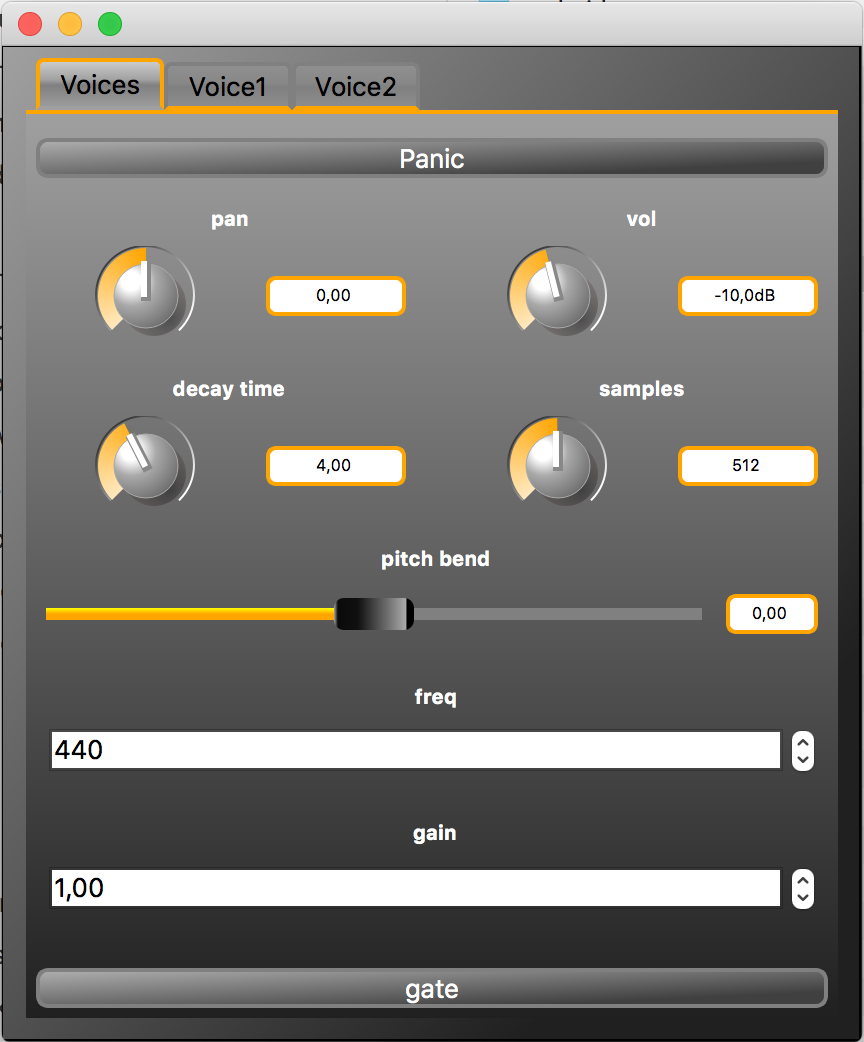
\includegraphics[width=0.6\columnwidth]{images/poly_ui}
\caption{\footnotesize Extended multi-voices GUI interface}
\label{fig:poly-ui}
\end{center}
\end{figure}

The resulting polyphonic DSP object can be used as usual, connected with the needed audio driver, and possibly other UI control objects like OSCUI, httpdUI, etc. Having this new UI hierarchical view allows complete OSC control of each single voice and their control parameters, but also all voices using the master component. 

The following OSC messages reflect the same DSP code either compiled normally,  or in polyphonic mode (only part of the OSC hierarchies are displayed here):

\footnotesize
\begin{lstlisting}

// Mono mode

/0x00/0x00/vol f -10.0
/0x00/0x00/pan f 0.0

// Polyphonic mode

/Polyphonic/Voices/0x00/0x00/pan f 0.0
/Polyphonic/Voices/0x00/0x00/vol f -10.0
...
/Polyphonic/Voice1/0x00/0x00/vol f -10.0
/Polyphonic/Voice1/0x00/0x00/pan f 0.0
...
/Polyphonic/Voice2/0x00/0x00/vol f -10.0
/Polyphonic/Voice2/0x00/0x00/pan f 0.0
...
\end{lstlisting}
\normalsize

The polyphonic instrument allocation takes the DSP to be used for one voice\footnote{The DSP object will be automatically cloned in the mydsp\_poly class to create all needed voices.},  the desired number of voices, the {\it dynamic voice allocation} state\footnote{Voices may be always running, or dynamically started/stopped in case of MIDI control.},  and the {\it group} state which controls if separated voices are displayed or not (Figure \ref{fig:poly-ui}): 

\footnotesize
\begin{lstlisting}
    DSP = new mydsp_poly(dsp, 2, true, true);  
\end{lstlisting}
    
\normalsize
With the following code, note that a polyphonic instrument may be used outside of a MIDI control context, so that all voices will be always running and possibly controlled with OSC messages for instance:

\footnotesize
\begin{lstlisting}
    DSP = new mydsp_poly(dsp, 8, false, true);
\end{lstlisting}

\normalsize
    
\section{Controlling the polyphonic instrument}

The \code{mydsp_poly} class is also ready for MIDI control and can react to {\it keyon/keyoff} and {\it pitchwheel} messages. Other MIDI control parameters can directly be added in the DSP source code. 

\section{Deploying the polyphonic instrument}

Several architecture files and associated scripts have been updated to handle polyphonic instruments:

As an example on OSX, the script \code{faust2caqt foo.dsp} can be used to create a polyphonic CoreAudio/QT application. The desired number of voices is either declared in a \code{nvoices} metadata or changed with the \code{-nvoices num} additional parameter\footnote{-nvoices parameter takes precedence over the  metadata value.}. MIDI control is activated using the \code{-midi} parameter. 

The number of allocated voices can possibly be changed at runtime using the \code{-nvoices} parameter to change the default value (so using \code{./foo -nvoices 16} for instance). 

Several other scripts have been adapted using the same conventions.

\section{Polyphonic instrument with a global output effect}

Polyphonic instruments may be used with an output effect. Putting that effect in the main \faust code is not a good idea since it would be instantiated for each voice which would be very inefficient. This is a typical use case for the  \code{dsp_sequencer} class previously presented with the polyphonic DSP connected in sequence with a unique global effect (Figure \ref{fig:poly-ui-effect}). 

\code{faustcaqt inst.dsp -effect effect.dsp} with inst.dsp and effect.dsp in the same folder,  and the number of outputs of the instrument matching the number of inputs of the effect, has to be used. A \code{dsp_sequencer} object will be created to combine the polyphonic instrument in sequence with the single output effect. 

Polyphonic ready  {\it faust2xx} scripts will then compile the polyphonic instrument and the effect, combine them in sequence, and create a ready to use DSP.  

\begin{figure}[!ht]
\begin{center}
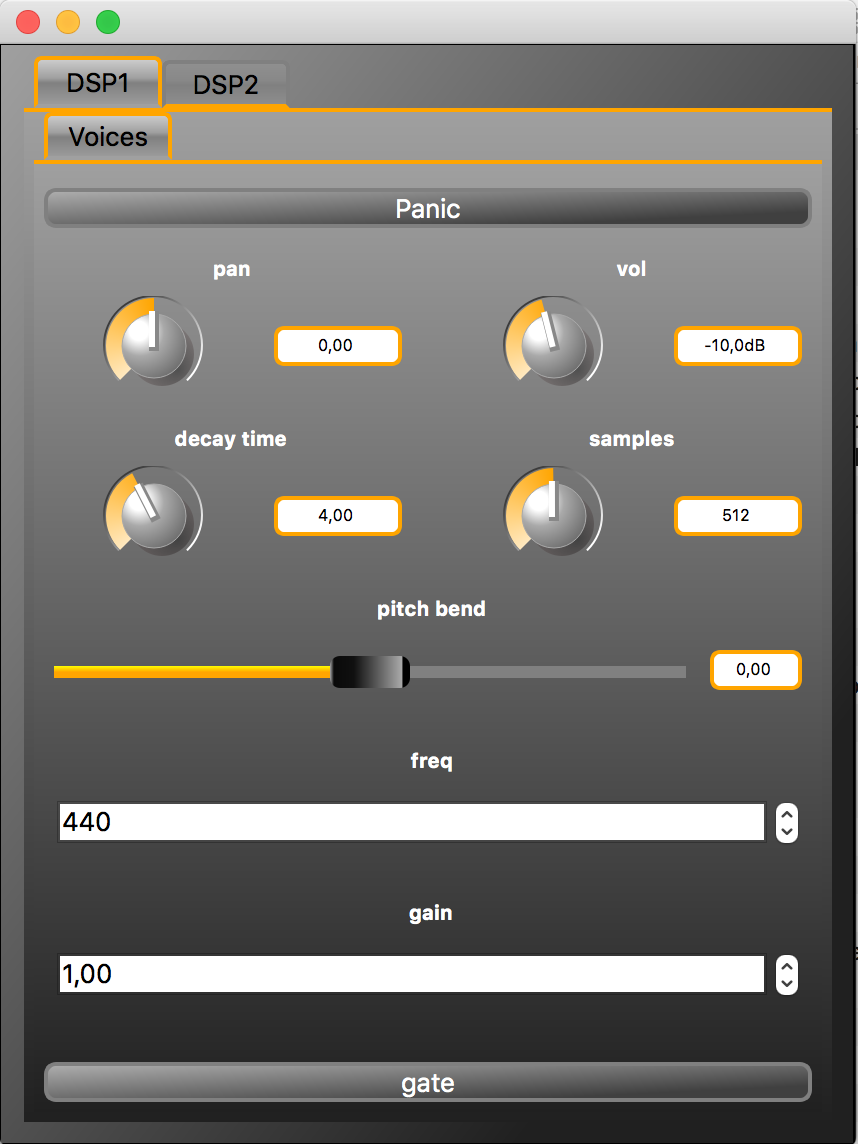
\includegraphics[width=0.48\columnwidth]{images/poly_ui_effect1}
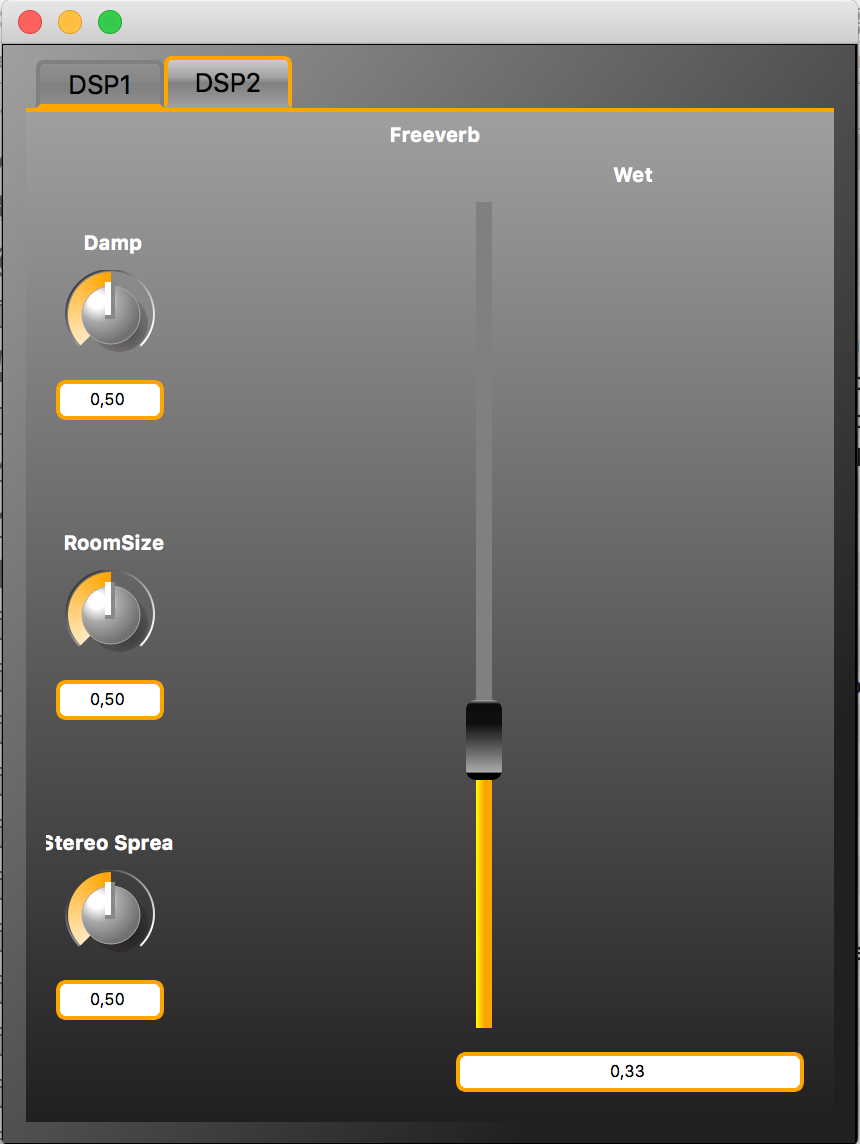
\includegraphics[width=0.48\columnwidth]{images/poly_ui_effect2}
\caption{\footnotesize Polyphonic instrument with output effect GUI interface: left tab window shows the polyphonic instrument with its {\it Voices} group only, right tab window shows the output effect.}
\label{fig:poly-ui-effect}
\end{center}
\end{figure}

\subsection{Integrated global output effect}

Starting with the 2.5.17 version, a new convention has been defined to directly integrate a global output effect inside the DSP source code itself. The effect has simply to be declared in a \code{effect =  effect_code;} line in the source. Here is a more complete source code example:

\begin{lstlisting}
import("stdfaust.lib");
process = pm.clarinet_ui_MIDI <: _,_;
effect = dm.freeverb_demo;
\end{lstlisting}

The architecture script then separate the instrument description itself (the \code{process = ...} definition) from the effect definition (the  \code{effect = ...} definition), possibly adapt the instrument number of outputs to the effect number of inputs, compile each part separately, and combine them with the \code{dsp_sequencer} object.

A new \code{auto} parameter to be used in faust2xx script has been defined, as in the \code{faustcaqt inst.dsp -effect auto} line for example.

\subsection{Integrated global output effect and libfaust}

For developers using the libfaust library, an helper file named \code{faust/dsp/poly-dsp-tools.h} is available. It defines an API to automatically create a polyphonic instrument with an output effect, starting from a DSP source file using the  effect \code{effect = ...} convention. The function \code{createPolyDSPFactoryFromString} or  \\ \code{createPolyDSPFactoryFromFile} must be used to create the polyphonic DSP factory. Next, the \code{createPolyDSPInstance} function creates the polyphonic object (a subclass of \code{dsp_poly} type) to be used like a regular \code{dsp} type object. 

After the DSP factory has been compiled, your application or plugin may want to save/restore it in order to save \faust to LLVM IR compilation or even JIT compilation time at next use. To get the internal factory compiled code, several functions are available:

\begin{itemize}
\item \code{writePolyDSPFactoryToIRFile} allows to save the polyphonic factory LLVM IR (in textual format) in a file,
\item \code{writePolyDSPFactoryToBitcodeFile} allows to save the polyphonic factory LLVM IR (in binary format) in a file,
\item \code{writePolyDSPFactoryToMachineFile} allows to save the polyphonic factory executable machine code in a file.
\end{itemize}

To re-create a DSP factory from a previously saved code, several functions are available:

\begin{itemize}
\item \code{readPolyDSPFactoryFromIRFile} allows to create a polyphonic DSP factory from a file containing the LLVM IR (in textual format),
\item \code{readPolyDSPFactoryFromBitcodeFile} allows to create a polyphonic  factory from a file containing the LLVM IR (in binary format),
\item \code{readPolyDSPFactoryFromMachineFile} allows to create a polyphonic DSP factory from a file containing the executable machine code.
\end{itemize}

\chapter{Controlling the code generation}
Several options of the \faust compiler allow to control the generated C++ code. By default the computations are done sample by sample in a single loop. But the compiler can also generate \textit{vector} and \textit{parallel} code.

\section{Vector code generation}
Modern C++ compilers are able to do autovectorization, that is to use SIMD instructions to speedup the code. These instructions can typically operate in parallel on short vectors of 4 simple precision floating point numbers thus leading to a theoretical speedup of $\times4$. 
Autovectorization of C/C++ programs is a difficult task. Current compilers are very sensitive to the way the code is arranged. In particular too complex loops can prevent autovectorization. The goal of the vector code generation is to rearrange the C++ code in a way that facilitates the autovectorization job of the C++ compiler. Instead of generating a single sample computation loop, it splits the computation into several simpler loops that communicates by vectors.

The vector code generation is activated by passing the \lstinline!--vectorize! (or \lstinline!-vec!) option to the \faust compiler. Two additional options are available:  \lstinline!--vec-size <n>! controls the size of the vector (by default 32 samples) and \lstinline!--loop-variant 0/1! gives some additional control on the loops.  

To illustrate the difference between scalar code and vector code, let's take the computation of the RMS (Root Mean Square) value of a signal.  Here is the \faust code that computes the Root Mean Square of a sliding window of 1000 samples:
\label{rms}
\begin{lstlisting}
// Root Mean Square of n consecutive samples
RMS(n) = square : mean(n) : sqrt;

// Square of a signal
square(x) = x * x;

// Mean of n consecutive samples of a signal
// (uses fixpoint to avoid the accumulation of
// rounding errors) 
mean(n) = float2fix : integrate(n) : 
          fix2float : /(n); 

// Sliding sum of n consecutive samples
integrate(n,x) = x - x@n : +~_;

// Convertion between float and fix point
float2fix(x) = int(x*(1<<20));      
fix2float(x) = float(x)/(1<<20);    

// Root Mean Square of 1000 consecutive samples
process = RMS(1000);
\end{lstlisting}

The compute() method generated in scalar mode is the following:

\begin{lstlisting}
virtual void compute (int count, 
                      float** input, 
                      float** output) 
{
  float* input0 = input[0];
  float* output0 = output[0];
  for (int i=0; i<count; i++) {
    float fTemp0 = input0[i];
    int iTemp1 = int(1048576*fTemp0*fTemp0);
    iVec0[IOTA&1023] = iTemp1;
    iRec0[0] = ((iVec0[IOTA&1023] + iRec0[1])
                    - iVec0[(IOTA-1000)&1023]);
    output0[i] = sqrtf(9.536744e-10f * 
                       float(iRec0[0]));
    // post processing
    iRec0[1] = iRec0[0];
    IOTA = IOTA+1;
  }
}
\end{lstlisting}

The \lstinline!-vec! option leads to the following reorganization of the code:
\begin{lstlisting}
virtual void compute (int fullcount, 
                      float** input, 
                      float** output) 
{
  int iRec0_tmp[32+4];
  int* iRec0 = &iRec0_tmp[4];
  for (int index=0; index<fullcount; index+=32) 
  {
    int count = min (32, fullcount-index);
    float* input0 = &input[0][index];
    float* output0 = &output[0][index];
    for (int i=0; i<4; i++) 
      iRec0_tmp[i]=iRec0_perm[i];
    // SECTION : 1
    for (int i=0; i<count; i++) {
      iYec0[(iYec0_idx+i)&2047] =
               int(1048576*input0[i]*input0[i]);
    }
    // SECTION : 2
    for (int i=0; i<count; i++) {
      iRec0[i] = ((iYec0[i] + iRec0[i-1]) - 
               iYec0[(iYec0_idx+i-1000)&2047]);
    }
    // SECTION : 3
    for (int i=0; i<count; i++) {
      output0[i] = sqrtf((9.536744e-10f * 
                 float(iRec0[i])));
    }
    // SECTION : 4
    iYec0_idx = (iYec0_idx+count)&2047;
    for (int i=0; i<4; i++)
      iRec0_perm[i]=iRec0_tmp[count+i];
  }
}
\end{lstlisting}

While the second version of the code is more complex, it turns out to be much easier to vectorize efficiently by the C++ compiler. Using Intel icc 11.0, with the exact same compilation options: \texttt{-O3 -xHost -ftz -fno-alias -fp-model fast=2}, the scalar version leads to a throughput performance of 129.144  MB/s, while the vector version achieves 359.548  MB/s, a speedup of x2.8 ! 

\begin{figure}[htb]
  \centering
  \includegraphics[scale=0.75]{images/compiler-stack}
  \caption{\faust's stack of code generators}   
  \label{fig:stack}
\end{figure}

The vector code generation is built on top of the scalar code generation (see figure \ref{fig:stack}). Every time an expression needs to be compiled, the compiler checks if it requires a separate loop or not. It applies some simple rules for that. Expressions that are shared (and are complex enough) are good candidates to be compiled in a separate loop, as well as recursive expressions and expressions used in delay lines. 

The result is a directed graph in which each node is a computation loop (see Figure \ref{fig:loopgraph}). This graph is stored in the klass object and a topological sort is applied to it before printing the code. 

\begin{figure}[htb]
  \centering
  \includegraphics[scale=0.75]{graphs/loopgraph2}
  \caption{The result of the -vec option is a directed acyclic graph (DAG) of small computation loops}   
  \label{fig:loopgraph}
\end{figure}

\section{Parallel code generation}

The parallel code generation is activated by passing either the \lstinline!--openMP! (or \lstinline!-omp!) option or the \lstinline!--scheduler! (or \lstinline!-sch!) option. It implies the \lstinline!-vec! options as the parallel code generation is built on top of the vector code generation.  

\subsection{The OpenMP code generator}

\begin{figure}[htb]
  \centering
  \includegraphics[scale=0.5,angle=-90]{images/openmp-model}
  \caption{OpenMP is based on a fork-join model}   
  \label{fig:openmp}
\end{figure}

The \lstinline!--openMP! (or \lstinline!-omp!) option given to the \faust compiler will insert appropriate OpenMP directives in the C++ code. OpenMP (http://wwww.openmp.org) is a well established API that is used to explicitly define direct multi-threaded, shared memory parallelism. It is based on a fork-join model of parallelism (see figure \ref{fig:openmp}). 
Parallel regions are delimited by \lstinline!#pragma omp parallel! constructs. At the entrance of a parallel region a team of parallel threads is activated. The code within a parallel region is executed by each thread of the parallel team until the end of the region. 

\begin{lstlisting}
#pragma omp parallel
{
  // the code here is executed simultaneously by 
  // every thread of the parallel team
  ...
}
\end{lstlisting}

In order not to have every thread doing redundantly the exact same work, OpemMP provides specific \textit{work-sharing} directives. For example \lstinline!#pragma omp sections! allows to break the work into separate, discrete sections, each section being executed by one thread:

\begin{lstlisting}
#pragma omp parallel
{
  #pragma omp sections
  {
    #pragma omp section
    {
      // job 1
    }
    #pragma omp section
    {
      // job 2
    }
    ...
  }

  ...
}
\end{lstlisting}

\subsection{Adding OpenMP directives}
As said before the parallel code generation is built on top of the vector code generation. The graph of loops produced by the vector code generator is topologically sorted in order to detect the loops that can be computed in parallel. The first set $S_0$ (loops $L1$, $L2$ and $L3$ in the DAG of Figure \ref{fig:loopgraph}) contains the loops that don't depend on any other loops, the set $S_1$ contains the loops that only depend on loops of $S_0$, (that is loops $L4$ and $L5$), etc.. 

As all the loops of a given set $S_n$ can be computed in parallel, the compiler will generate a \lstinline!sections! construct with a \lstinline!section! for each loop. 
\begin{lstlisting}
  #pragma omp sections
  {
    #pragma omp section
    for (...) {
      // Loop 1
    }
    #pragma omp section
    for (...) {
      // Loop 2
    }
    ...
  }
\end{lstlisting}
 
If a given set contains only one loop, then the compiler checks to see if the loop can be parallelized (no recursive dependencies) or not. If it can be parallelized, it generates:
\begin{lstlisting}
  #pragma omp for
  for (...) {
   // Loop code
  }
\end{lstlisting}
otherwise it generates a \lstinline!single! construct so that only one thread will execute the loop:
\begin{lstlisting}
  #pragma omp single
  for (...) {
   // Loop code
  }
\end{lstlisting}

\subsection{Example of parallel OpenMP code}
To illustrate how \faust uses the OpenMP directives, here is a very simple example, two 1-pole filters in parallel connected to an adder (see figure \ref{fig:parfilter} the corresponding block-diagram):

\begin{lstlisting}
filter(c) = *(1-c) : + ~ *(c);
process = filter(0.9), filter(0.9) : +; 
\end{lstlisting}

\begin{figure}[htb] 
  \centering
  \includegraphics[width=8cm]{images/filter2}
  \caption{two filters in parallel connected to an adder}   
  \label{fig:parfilter}
\end{figure}

The corresponding compute() method obtained using the \lstinline!-omp! option is the following:
\begin{lstlisting}

virtual void compute (int fullcount, 
                      float** input, 
                      float** output) 
{
  float   fRec0_tmp[32+4];
  float   fRec1_tmp[32+4];
  float*  fRec0 = &fRec0_tmp[4];
  float*  fRec1 = &fRec1_tmp[4];
  #pragma omp parallel firstprivate(fRec0,fRec1)
  {
    for (int index = 0; index < fullcount; 
                                index += 32) 
    {
      int count = min (32, fullcount-index);
      float* input0 = &input[0][index];
      float* input1 = &input[1][index];
      float* output0 = &output[0][index];
      #pragma omp single
      {
        for (int i=0; i<4; i++) 
          fRec0_tmp[i]=fRec0_perm[i];
        for (int i=0; i<4; i++) 
          fRec1_tmp[i]=fRec1_perm[i];
      }
      // SECTION : 1
      #pragma omp sections
      {
        #pragma omp section
        for (int i=0; i<count; i++) {
          fRec0[i] = ((0.1f * input1[i]) 
                   + (0.9f * fRec0[i-1]));
        }
        #pragma omp section
        for (int i=0; i<count; i++) {
          fRec1[i] = ((0.1f * input0[i]) 
                   + (0.9f * fRec1[i-1]));
        }
      }
      // SECTION : 2
      #pragma omp for
      for (int i=0; i<count; i++) {
        output0[i] = (fRec1[i] + fRec0[i]);
      }
      // SECTION : 3
      #pragma omp single
      {
        for (int i=0; i<4; i++) 
          fRec0_perm[i]=fRec0_tmp[count+i];
        for (int i=0; i<4; i++) 
          fRec1_perm[i]=fRec1_tmp[count+i];
      }
    }
  }
}

\end{lstlisting}

This code requires some comments:

\begin{enumerate}
\item The parallel construct \lstinline!#pragma omp parallel! is the fundamental construct that starts parallel execution. The number of parallel threads is generally the number of CPU cores but it can be controlled in several ways.

\item Variables external to the parallel region are shared by default. The pragma \lstinline!firstprivate(fRec0,fRec1)! indicates that each thread should have its private copy of fRec0 and fRec1. The reason is that accessing shared variables requires an indirection and is quite inefficient compared to private copies.

\item The top level loop \lstinline!for (int index = 0;...)...! is executed by all threads simultaneously. The subsequent work-sharing directives inside the loop will indicate how the work must be shared between the threads. 

\item Please note that an implied barrier exists at the end of each work-sharing region. All threads must have executed the barrier before any of them can continue.

\item The work-sharing directive \lstinline!#pragma omp single! indicates that this first section will be executed by only one thread (any of them).

\item The work-sharing directive \lstinline!#pragma omp sections! indicates that each corresponding \lstinline!#pragma omp section!, here our two filters, will be executed in parallel.

\item The loop construct \lstinline!#pragma omp for! specifies that the iterations of the associated loop will be executed in parallel. The iterations of the loop are distributed across the parallel threads. For example, if we have two threads, the first one can compute indices between 0 and count/2 and the other one between count/2 and count. 

\item Finally \lstinline!#pragma omp single!  in section 3 indicates that this last section will be executed by only one thread (any of them).

\end{enumerate}

\subsection{The scheduler code generator}
 With the \lstinline!--scheduler! (or \lstinline!-sch!) option given to the \faust compiler, the computation graph is cut into separated computation loops (called "tasks"), and a "Work Stealing Scheduler" is used to activate and execute them following their dependencies. A pool of worked threads is created and each thread uses it's own local WSQ (Work Stealing Queue) of tasks. A WSQ is a special queue with a Push operation, a "private" LIFO Pop operation and a "public" FIFO Pop operation.

Starting from a ready task, each thread follows the dependencies, possibly pushing ready sub-tasks into it's own local WSQ. When no more tasks can be activated on a given computation path, the thread pops a task from it's local WSQ. If the WSQ is empty, then the thread is allowed to "steal" tasks from other threads WSQ.

The local LIFO Pop operation allows better cache locality and the FIFO steal Pop "larger chuck" of work to be done. The reason for this is that many work stealing workloads are divide-and-conquer in nature, stealing one of the oldest task implicitly also steals a (potentially) large subtree of computations that will unfold once that piece of work is stolen and run.

Compared to the OpenMP model (\lstinline!-omp!) the new model is worse for simple \faust  programs and usually starts to behave comparable or sometimes better for "complex enough" \faust  programs. In any case, since OpenMP does not behave so well with GCC compilers (only quite recent versions like GCC 4.4 start to show some improvements), and is unusable on OSX in real-time contexts, this new scheduler option has it's own value.  We plan to improve it adding a "pipelining" idea in the future.

\subsection{Example of parallel scheduler code}
To illustrate how \faust generates the scheduler code, here is a very simple example, two 1-pole filters in parallel connected to an adder (see figure \ref{fig:parfilter} the corresponding block-diagram):

\begin{lstlisting}
filter(c) = *(1-c) : + ~ *(c);
process = filter(0.9), filter(0.9) : +; 
\end{lstlisting}


When \lstinline!-sch! option is used, the content of the additional \textit{architecture/scheduler.h} file is inserted in the generated code. It contains code to deal with WSQ and thread management. The \lstinline'compute()' and \lstinline'computeThread()' methods are the following:
\begin{lstlisting}

virtual void compute (int fullcount, 
                      float** input, 
                      float** output) 
{
	GetRealTime();
	this->input = input;
	this->output = output;
	StartMeasure();
	for (fIndex = 0; fIndex < fullcount; fIndex += 32) {
		fFullCount = min (32, fullcount-fIndex);
		TaskQueue::Init();
		// Initialize end task
		fGraph.InitTask(1,1);
		// Only initialize tasks with inputs
		fGraph.InitTask(4,2);
		fIsFinished = false;
		fThreadPool.SignalAll(fDynamicNumThreads - 1);
		computeThread(0);
		while (!fThreadPool.IsFinished()) {}
	}
	StopMeasure(fStaticNumThreads, 
		fDynamicNumThreads);
}
void computeThread (int cur_thread) {
	float* 	fRec0 = &fRec0_tmp[4];
	float* 	fRec1 = &fRec1_tmp[4];
	// Init graph state
	{
		TaskQueue taskqueue;
		int tasknum = -1;
		int count = fFullCount;
		// Init input and output
		FAUSTFLOAT* input0 = &input[0][fIndex];
		FAUSTFLOAT* input1 = &input[1][fIndex];
		FAUSTFLOAT* output0 = &output[0][fIndex];
		int task_list_size = 2;
		int task_list[2] = {2,3};
		taskqueue.InitTaskList(task_list_size, task_list, fDynamicNumThreads, cur_thread, tasknum);
		while (!fIsFinished) {
			switch (tasknum) {
				case WORK_STEALING_INDEX: { 
					tasknum = TaskQueue::GetNextTask(cur_thread);
					break;
				} 
				case LAST_TASK_INDEX: { 
					fIsFinished = true;
					break;
				} 
				// SECTION : 1
				case 2: { 
					// LOOP 0x101111680
					// pre processing
					for (int i=0; i<4; i++) fRec0_tmp[i]=fRec0_perm[i];
					// exec code
					for (int i=0; i<count; i++) {
						fRec0[i] = ((1.000000e-01f * (float)input1[i]) + (0.9f * fRec0[i-1]));
					}
					// post processing
					for (int i=0; i<4; i++) fRec0_perm[i]=fRec0_tmp[count+i];
					
					fGraph.ActivateOneOutputTask(taskqueue, 4, tasknum);
					break;
				} 
				case 3: { 
					// LOOP 0x1011125e0
					// pre processing
					for (int i=0; i<4; i++) fRec1_tmp[i]=fRec1_perm[i];
					// exec code
					for (int i=0; i<count; i++) {
						fRec1[i] = ((1.000000e-01f * (float)input0[i]) + (0.9f * fRec1[i-1]));
					}
					// post processing
					for (int i=0; i<4; i++) fRec1_perm[i]=fRec1_tmp[count+i];
					
					fGraph.ActivateOneOutputTask(taskqueue, 4, tasknum);
					break;
				} 
				case 4: { 
					// LOOP 0x101111580
					// exec code
					for (int i=0; i<count; i++) {
						output0[i] = (FAUSTFLOAT)(fRec1[i] + fRec0[i]);
					}
					
					tasknum = LAST_TASK_INDEX;
					break;
				} 
			}
		}
	}
}

\end{lstlisting}
  
\input{chapters/mathdoc} 
\chapter{Acknowledgments}
Many persons are contributing to the \faust project, by providing code for the compiler, architecture files, libraries, examples, documentation, scripts, bug reports, ideas, etc. We would like in particular to thank:

\begin{itemize}
\item[-]Fons Adriaensen	
\item[-]Karim Barkati
\item[-]J\'er\^ome Barth\'elemy
\item[-]Tim Blechmann
\item[-]Tiziano Bole	
\item[-]Alain Bonardi
\item[-]Thomas Charbonnel
\item[-]Raffaele Ciavarella
\item[-]Julien Colafrancesco
\item[-]Damien Cramet
\item[-]\'Etienne Gaudrin
\item[-]Pierre Guillot
\item[-]Albert Gr\"af
\item[-]Pierre Jouvelot
\item[-]Stefan Kersten
\item[-]Victor Lazzarini
\item[-]Matthieu Leberre
\item[-]Mathieu Leroi
\item[-]Fernando Lopez-Lezcano
\item[-]Kjetil Matheussen
\item[-]Hermann Meyer
\item[-]Romain Michon
\item[-]R\'emy Muller
\item[-]Eliott Paris
\item[-]Reza Payami
\item[-]Laurent Pottier
\item[-]Sampo Savolainen
\item[-]Nicolas Scaringella
\item[-]Anne Sedes
\item[-]Priyanka Shekar
\item[-]Stephen Sinclair
\item[-]Travis Skare
\item[-]Julius Smith
\item[-]Michael Wilson
\end{itemize}
as well as our colleagues at GRAME:
\begin{itemize}
\item[-]Sarah Denoux
\item[-]Dominique Fober
\item[-]Olivier Guillerminet
\item[-]Christophe Lebreton
\item[-]St\'ephane Letz
\item[-]Mike Solomon
\end{itemize}

We would like also to thank for their financial support:
\begin{itemize}
\item[-]the French Ministry of Culture
\item[-]the Rh\^one-Alpes Region
\item[-]the City of Lyon
\item[-]the French National Research Agency (\textsc{ANR})
\end{itemize}


 

\end{document}
